\documentclass[12pt]{report}

% Paquetes LaTeX y estilos globales
\input{etc/pkgs}
\input{etc/style}

%%%%%%%%%%%%%%%%%%%%%%%%%%%%%%%%%%%%%%%%%%%%%%%%%%%%%%%%%%%%%%%%%%%%%%%%%%%%%%%%%%%%%

% Variables para la portada
\setTitle{GlucoMate \\ \medskip \textit{Gestión inteligente y monitorización en tiempo real para tu diabetes.}}
\setAuthor{Manuel Ortega García} % Si hay más de un autor, separarlos con \\
\setDegree{Grado en Ingeniería Informática - Ingeniería del Software} % Cambiar si es necesario
\setSupervisor{Manuel Jesus Domínguez Morales \\ Luis Muñoz Saavedra} % Si hay más de un tutor, separarlos con \\
\setDepartment{Arquitectura y Tecnología de Computadores}
\setMonth{junio} % Dejar sólo el mes de la convocatoria en que se presenta el trabajo
\setYear{2025/26} % Por ejemplo, 2022/23

%%%%%%%%%%%%%%%%%%%%%%%%%%%%%%%%%%%%%%%%%%%%%%%%%%%%%%%%%%%%%%%%%%%%%%%%%%%%%%%%%%%%%

% Dedicatoria del trabajo
% Si no se desea incluir, comentar o borrar la línea siguiente para eliminar la página de dedicatoria
\setDedication{Dedicado a mis padres y a mi hermana, quienes siempre me han mantenido enfocado en lo que hago y en lo que puedo llegar a ser. Por hacerme fuerte cuando mas débil he sido.\\ Gracias sois mi vida.\\[10pt]
Y a mi pareja que empezó conmigo esta etapa de mi vida y me acompaña a cerrarla.\\ Te quiero.\\[10pt]

Os los dedico\\[20pt]

Cuando el aire era más puro\\
y la marisma más verde.\\
Cuando al nacer la mañana\\
volaban patos silvestres.\\
Cuando el coto de Doñana\\
era alfombra celeste\\
y el cielo se reflejaba\\
en los lucios transparentes.\\[5pt]

Completamente redondo\\
estaba el sol amarillo,\\
que besaba el horizonte\\
bañándolo con su brillo.\\
Las nubes tímidamente\\
se teñían de naranja\\
y se alargaban las sombras\\
de los pinos verde y malva.\\[5pt]

Rompió el silencio de siglos\\
un ladrido en la Rocina.\\
Junto un reseco acebuche\\
los perros se arremolinan.\\
Por el viejo tronco asoma\\
una cara tan divina,\\
que el cazaó emocionao\\
cayó al suelo de rodillas.\\[5pt]

Quien hubiera sido tú,\\
cazador de las marismas,\\
para quedar sorprendío\\
y ser el primero en ver\\
a la virgen del roció.\\

}

%%%%%%%%%%%%%%%%%%%%%%%%%%%%%%%%%%%%%%%%%%%%%%%%%%%%%%%%%%%%%%%%%%%%%%%%%%%%%%%%%%%%%

% Comienzo del documento
\begin{document}

    % Portada y secciones no numeradas
    \input{sections/00_portada}
    \chapter*{Agradecimientos}
Quisiera expresar mi más sincero agradecimiento a \textbf{Luis Muñoz Saavedra}, por haberme tutorizado y acompañado durante el desarrollo de este Trabajo de Fin de Grado. Su dedicación, orientación y apoyo constante han sido fundamentales para que este trabajo haya llegado a buen puerto y para que este proceso haya resultado tan enriquecedor y bonito.

Asimismo, quiero agradecer a \textbf{Manuel Jesús Domínguez Morales}, por haber sido mi tutor de TFG y por su disposición, ayuda y orientación a lo largo de este camino académico.

También quiero dar las gracias a mis compañeros de carrera y amigos, \textbf{Pepe, Luis, Juan Jesús y Analu}, por haber sido una fuente constante de motivación para seguir adelante en este gremio. Gracias por hacer los días más amenos, tanto durante la etapa universitaria como en el ámbito laboral, y por compartir conmigo tantos momentos que han hecho este camino mucho más llevadero.

Por último, quiero agradecer a mis amigos de toda la vida, por aguantar con paciencia todas las clases improvisadas de informática que les he dado, aunque en muchas ocasiones no fueran más que una excusa para repasar apuntes en voz alta. Gracias por vuestra paciencia, vuestro apoyo y por estar siempre ahí.
    \chapter*{Resumen}
Este proyecto desarrolla un ecosistema digital para la monitorización glucémica y la educación terapéutica mediante la integración de tecnología NFC (Near Field Communication) y Sistemas de Soporte a la Decisión (CDSS). El sistema permite la adquisición de datos de glucosa intersticial en tiempo real al conectarse directamente con sensores de monitorización continua (FreeStyle Libre 2 Plus), centralizando registros críticos como el perfil insulínico, las pautas médicas, la ingesta de carbohidratos y la actividad física.

El núcleo innovador del proyecto reside en una interfaz conversacional basada en Inteligencia Artificial Generativa (modelo tipo GPT). Este módulo actúa como un asistente pedagógico que analiza variables en tiempo real, como la Insulina Activa (IOB), para ofrecer orientaciones personalizadas ante situaciones de riesgo, incluyendo la prevención de hipoglucemias tras el ejercicio o la gestión de la insulina basal.

Bajo un enfoque estrictamente educativo, el objetivo principal es empoderar al usuario sin conocimientos previos, permitiéndole afianzar conceptos y aprender de forma intuitiva a través de sus propios datos. El sistema prioriza la seguridad, contextualizando cada respuesta de la IA como un soporte complementario que refuerza, y no sustituye, las pautas médicas establecidas. En definitiva, el proyecto demuestra cómo la convergencia de la monitorización biométrica y la IA facilita una comprensión más profunda y accesible de la gestión diaria de la diabetes.
\vspace{.5cm}

\textbf{Palabras clave:} Diabetes Mellitus, Inteligencia Artificial Generativa, Monitorización Continua de Glucosa (MCG), NFC, Sistemas de Soporte a la Decisión Clínica, Educación Terapéutica, mHealth.
    \chapter*{Abstract}
This project develops a digital ecosystem for glycemic monitoring and therapeutic education by integrating Near Field Communication (NFC) technology and Clinical Decision Support Systems (CDSS). The system enables real-time interstitial glucose data acquisition by connecting directly to continuous monitoring sensors (FreeStyle Libre 2 Plus), centralizing critical records such as insulin profiles, medical guidelines, carbohydrate intake, and physical activity.

The innovative core of the project lies in a conversational interface based on Generative Artificial Intelligence (GPT-style model). This module functions as a pedagogical assistant that analyzes real-time variables, such as Insulin on Board (IOB), to provide personalized guidance in risk situations, including the prevention of post-exercise hypoglycemia or the management of basal insulin.

With a strictly educational focus, the primary objective is to empower users without prior knowledge, allowing them to consolidate concepts and learn intuitively through their own data. The system prioritizes safety by contextualizing every AI response as complementary support that reinforces, rather than replaces, established medical guidelines. Ultimately, this project demonstrates how the convergence of biometric monitoring and AI facilitates a deeper and more accessible understanding of daily diabetes management.
\vspace{.5cm}

\textbf{Keywords:} Diabetes Mellitus, Generative Artificial Intelligence, Continuous Glucose Monitoring (CGM), NFC, Clinical Decision Support Systems (CDSS), Patient Education, mHealth.
    
    % Índice del documento y de figuras
    \begingroup
        % Los enlaces son normalmente azules, pero en los índices se configuran a negro para que no aparezca todo azul
        \hypersetup{linkcolor=black}
        \tableofcontents
        \listoffigures
        \listoftables
        \lstlistoflistings
    \endgroup
    
    % Cambia el estilo de números de página de romanos a normal
    \clearpage\pagenumbering{arabic}
    
    % Capítulos del trabajo

    % ============================================================
%  CAPÍTULO 1 — INTRODUCCIÓN
%  TFG: GlucoMate — Aplicación de Monitorización Continua de Glucosa
%  Ingeniería de Software
% ============================================================

\chapter{Introducción}
\label{cap:introduccion}

\section{Contexto}
\label{sec:contexto}

La diabetes mellitus tipo 1 (DM1) es una enfermedad crónica autoinmune en la que el
páncreas pierde de forma irreversible la capacidad de producir insulina, la hormona
responsable de regular la glucosa en sangre. Quienes la padecen deben sustituir
manualmente esa función pancreática: midiendo su glucosa varias veces al día, calculando
las dosis de insulina que necesitan antes de cada comida y tomando decisiones clínicas en
tiempo real a partir de esos datos. Un error en ese proceso puede desencadenar desde
una hipoglucemia leve —con síntomas de mareo, sudoración y confusión— hasta situaciones
potencialmente mortales como un coma diabético o una cetoacidosis.

\section{Motivación}
\label{sec:motivación}
La motivación de este proyecto es \negritas{profundamente personal} y nace de mi propia experiencia diaria conviviendo con la diabetes. Como paciente, identifico de primera mano las carencias de las soluciones actuales: mientras que aplicaciones oficiales como la del sistema FreeStyle Libre se limitan a una captura de datos básica y lineal, por otro lado, las alternativas existentes en el mercado suelen presentar barreras de acceso debido a su coste o carecen de un equilibrio entre simplicidad, usabilidad y funcionalidad, factores esenciales para pacientes con pocos conocimientos técnicos o recién diagnosticados. Esta realidad genera una frustración constante, ya que nos encontramos con herramientas que registran cifras, pero que no ofrecen un soporte real ante la incertidumbre del día a día.

Como usuario y paciente directamente afectado, mi impulso es crear la herramienta que considero que falta en el mercado: una plataforma que combine simplicidad, usabilidad y funcionalidad máxima. Mi objetivo es que cualquier persona con diabetes, independientemente de sus conocimientos tecnológicos o médicos, pueda entender su metabolismo y gestionar su enfermedad sin la carga cognitiva que supone interpretar datos aislados.

Desde \negritas{la perspectiva de la ingeniería}, el reto que me he propuesto es transformar esta necesidad vital en una solución tecnológica integral "Full Stack". El proyecto supone para mí un desafío de integración multidisciplinar: desde la interacción directa con el hardware del móvil mediante el chip NFC, hasta el diseño de una arquitectura completa que incluya Frontend, Backend y gestión de bases de datos, culminando con la integración de Inteligencia Artificial como motor de ayuda pedagógica. En definitiva, mi motivación reside en poner la ingeniería al servicio del paciente, facilitando una gestión de la diabetes más humana, inteligente y, sobre todo, accesible.

% ──────────────────────────────────────────────────────────────
\section{Objetivos del proyecto}
\label{sec:objetivos}

El objetivo general del proyecto es diseñar, implementar y validar \textbf{GlucoMate},
una aplicación móvil Android para la monitorización continua de glucosa, orientada a
pacientes con diabetes mellitus tipo 1 que utilizan el sensor Abbott Freestyle Libre 2
Plus.

Para alcanzar ese objetivo general se definen los siguientes \textbf{objetivos
específicos}:

\begin{enumerate}
    \item Integrar la lectura de datos del sensor Freestyle Libre 2 Plus en una
          aplicación React Native mediante el protocolo NFC, utilizando la aplicación
          Juggluco como puente de descifrado de la señal Bluetooth Low Energy (BLE)
          del sensor.

    \item Implementar un backend REST con Node.js y Express que persista las lecturas
          de glucosa y los eventos clínicos (insulina, comidas y ejercicio) en una
          base de datos PostgreSQL.

    \item Desarrollar una interfaz gráfica avanzada que muestre la curva histórica de
          glucosa de las últimas doce horas, con superposición de eventos clínicos,
          mediante la librería D3.js renderizada sobre SVG nativo en React Native.

    \item Crear un agente de inteligencia artificial,
          conociendo el estado glucémico actual del usuario, su
          insulina activa (IOB), su perfil de tratamiento y los deportes practicados
          recientemente, sea capaz de calcular dosis de insulina para una comida y
          ofrecer recomendaciones clínicas personalizadas.

    \item Diseñar una pantalla de perfil de usuario que permita configurar los
          parámetros individuales de tratamiento (insulinas, ratios ICR por franja
          horaria y factor de sensibilidad a la insulina FSI) que el agente de IA
          utiliza como contexto.

    \item Validar el sistema de forma integral con un sensor real Freestyle Libre 2
          Plus en un dispositivo Android físico.
\end{enumerate}

% ──────────────────────────────────────────────────────────────
\section{Alcance y limitaciones}
\label{sec:alcance}

GlucoMate es una aplicación de apoyo al autocontrol de la diabetes. No es un
producto sanitario certificado según el Reglamento Europeo de Productos Sanitarios
(MDR 2017/745) ni pretende serlo. Todas las recomendaciones que genera el agente de IA
se muestran acompañadas de un aviso explícito que indica que no reemplazan el criterio
clínico de un profesional de la salud.

En cuanto al alcance técnico, el proyecto cubre:

\begin{itemize}
    \item La capa móvil (frontend) completa: interfaz de usuario, lógica de presentación,
          comunicación con el backend y renderizado de la gráfica.
    \item La capa de servidor (backend): API REST, acceso a la base de datos y
          comunicación con la API de Groq para inferencia del modelo
          \texttt{llama-3.3-70b-versatile}.
    \item La base de datos relacional: esquema completo de tablas para glucosa, perfil
          de usuario, eventos de insulina, comidas y ejercicio.
\end{itemize}

Quedan fuera del alcance de esta versión:

\begin{itemize}
    \item El soporte para dispositivos iOS, dado que Apple restringe el acceso a NFC en
          modo de escritura y lectura ISO 15693 a aplicaciones certificadas por Abbott.
    \item La comunicación directa con el sensor sin Juggluco: en el estado actual de la
          ingeniería inversa del protocolo BLE del Freestyle Libre 2 Plus, el descifrado
          del enlace cifrado requiere el uso de esta aplicación intermediaria.
    \item Funcionalidades avanzadas como el cálculo automatizado de HbA1c estimada,
          el Tiempo en Rango (TiR) o la sincronización con la nube, identificadas como
          trabajo futuro.

\end{itemize}

% ──────────────────────────────────────────────────────────────
\section{Estructura del documento}
\label{sec:estructura}

La presente memoria se organiza en los siguientes capítulos:

\begin{description}
    \item[\textbf{Capítulo 2 — Estado del Arte.}] Analiza el contexto médico y tecnológico
    del proyecto: la diabetes tipo 1, los sistemas de monitorización continua de glucosa
    comerciales, el sensor Abbott Freestyle Libre 2 Plus, los proyectos de código abierto
    que han explorado la ingeniería inversa de sus protocolos (xDrip+, LibreMonitor,
    Juggluco) y las soluciones de inteligencia artificial aplicadas a la gestión de la
    diabetes.

    \item[\textbf{Capítulo 3 — Análisis del Problema.}] Recoge los requisitos funcionales
    y no funcionales del sistema, los actores implicados y los casos de uso principales,
    así como el modelo de dominio del problema.

    \item[\textbf{Capítulo 4 — Metodología de Desarrollo.}] Describe el proceso de trabajo
    seguido durante el proyecto: metodología ágil, control de versiones con Git y GitHub,
    uso de Conventional Commits y las buenas prácticas de desarrollo aplicadas.

    \item[\textbf{Capítulo 5 — Diseño de la Solución.}] Presenta la arquitectura general
    del sistema, el diseño de cada módulo, el esquema de la base de datos y los diagramas
    de componentes, secuencia y flujo de datos.


    \item[\textbf{Capítulo 6— Pruebas.}] Describe la estrategia de validación del sistema
    y los resultados obtenidos con el sensor real en un dispositivo Android físico.

    \item[\textbf{Capítulo 7 — Conclusiones y Trabajo Futuro.}] Evalúa el grado de
    cumplimiento de los objetivos, extrae las lecciones aprendidas y propone las líneas
    de mejora para versiones futuras.

    \item[\textbf{Bibliografía y Anexos.}] Referencias utilizadas a lo largo del documento
    y material complementario (fragmentos de código anotados, glosario).
\end{description}

    \chapter{Estado del arte}
\label{cap:estado-arte}

\section{La diabetes mellitus tipo 1 y el monitoreo continuo de glucosa}

La diabetes mellitus tipo 1 es una patología crónica en la que el organismo deja de
producir insulina, lo que obliga al paciente a tomar decisiones terapéuticas de forma
continua. En el día a día esto se traduce en medir la glucosa, calcular dosis de
insulina, estimar hidratos de carbono y anticipar el efecto del ejercicio. El problema no
es únicamente clínico, sino también informacional: el usuario debe interpretar datos muy
heterogéneos en un intervalo temporal corto.

Los sistemas de monitorización continua de glucosa suponen un salto cualitativo frente a
la glucemia capilar tradicional, ya que permiten disponer de un valor reciente de glucosa
intersticial y, además, de una tendencia de evolución. Esa combinación de valor actual,
histórico y dirección de cambio hace posible detectar hipoglucemias, hiperglucemias o
subidas rápidas antes de que el problema sea evidente desde una única medición aislada.

Sin embargo, disponer de más datos no resuelve por sí mismo la dificultad de gestión. El
usuario sigue necesitando relacionar esas lecturas con la insulina administrada, la comida
ingerida y la actividad física realizada. Precisamente ahí aparece el hueco que pretende
cubrir GlucoMate: no solo leer glucosa, sino contextualizarla.

\section{Sistemas CGM comerciales: Abbott Freestyle Libre}

Dentro de los sistemas comerciales de CGM (\textbf{monitoreo continuo de glucosa}), la familia \textit{Freestyle Libre} se ha
consolidado como una de las más extendidas por su facilidad de uso y por la integración
con teléfonos móviles. El sensor se adhiere al brazo y permite recuperar datos de glucosa
mediante tecnologías inalámbricas, principalmente NFC para ciertas interacciones de
lectura y Bluetooth Low Energy para la comunicación continuada en modelos recientes.

Para este proyecto, el sensor de referencia es el \textit{Freestyle Libre 2 Plus}. La
elección no es casual: es un dispositivo ampliamente utilizado, con una comunidad activa
de usuarios y desarrolladores interesados en comprender su funcionamiento más allá del
ecosistema oficial. Además, representa un caso realista de integración entre hardware
médico, protocolos propietarios y aplicaciones móviles de terceros.

La principal limitación del entorno comercial no es la capacidad de medición, sino el
grado de apertura. Las aplicaciones oficiales priorizan la seguridad del ecosistema y la
experiencia cerrada del fabricante, pero ofrecen poca flexibilidad para integrar la señal
glucémica con otros datos generados por el paciente o para experimentar con nuevas capas
de análisis. GlucoMate se plantea precisamente como una alternativa investigadora sobre
esa base tecnológica.

\section{Aplicaciones existentes: xDrip+, LibreMonitor, Glimp}

Antes de plantear una solución propia es necesario analizar las herramientas ya
existentes. Proyectos como \textit{xDrip+}, \textit{LibreMonitor} o \textit{Glimp} han
demostrado que existe un interés real en ampliar las posibilidades de los sensores Abbott
mediante software no oficial. Estas aplicaciones destacan por ofrecer funciones de
visualización avanzada, alarmas, exportación de datos o integración con otros servicios.

No obstante, muchas de ellas están orientadas a perfiles de usuario avanzados, requieren
configuraciones técnicas poco amigables o se centran en un subconjunto del problema.
Algunas sobresalen en conectividad, otras en comunidad, y otras en soporte histórico, pero
no todas ofrecen un equilibrio adecuado entre simplicidad de uso, registro clínico,
persistencia estructurada e interpretación pedagógica de los datos.

La oportunidad de GlucoMate no consiste en replicar exactamente esas herramientas, sino
en combinar varias ideas valiosas en una propuesta cohesionada: lectura de glucosa,
registro de comidas, insulina y ejercicio, perfil terapéutico configurable y un agente de
apoyo basado en IA capaz de usar ese contexto de manera integrada.

\section{Ingeniería inversa del protocolo Abbott}

Uno de los aspectos más relevantes del estado del arte en este proyecto es el trabajo de
ingeniería inversa realizado por la comunidad sobre los sensores de Abbott. Aunque el
transporte físico puede apoyarse en estándares conocidos, como ISO~15693 en el ámbito NFC
o BLE en la comunicación continua, la semántica de determinados comandos y el formato de
los datos no forman parte de una documentación pública orientada a desarrolladores de
terceros.

Como parte del análisis experimental se realizó un intento de lectura directa del sensor
\textit{Freestyle Libre 2 Plus} desde un dispositivo Android. Desde el punto de vista de
hardware, el sensor expone una interfaz compatible con NFC-V, tecnología asociada al
estándar ISO~15693. El objetivo de esta prueba era validar si un teléfono móvil podía
establecer comunicación con el parche, identificarlo correctamente y acceder a sus
bloques de memoria mediante comandos NFC estándar.

Para esta primera aproximación se utilizó React Native junto con Expo. Sin embargo, se
comprobó que la aplicación estándar Expo Go no resultaba suficiente para este caso de
uso, ya que no incorpora los módulos nativos necesarios para acceder a la antena NFC del
dispositivo Android. Por este motivo, fue necesario plantear una \textit{Development
Build} mediante EAS Build, incorporando la librería \texttt{react-native-nfc-manager} y
los permisos específicos de Android requeridos para el uso de NFC.

Durante la puesta en marcha del entorno de pruebas apareció una dificultad adicional
relacionada con la conexión entre la aplicación instalada en el móvil y el servidor de
desarrollo Metro. El APK intentaba resolver \texttt{localhost} o \texttt{127.0.0.1} desde
el propio dispositivo Android, lo que impedía alcanzar el servidor ejecutado en el
ordenador. A esto se sumaban posibles restricciones de red, como el cortafuegos de
Windows o la falta de visibilidad entre direcciones IP de la red local. Para resolverlo
se utilizó ADB como puente de depuración mediante USB. Tras autorizar el dispositivo, se
redirigió el puerto de Metro con el comando \texttt{adb reverse tcp:8081 tcp:8081} y se
lanzó Expo en modo local. De esta forma, las peticiones realizadas por la aplicación a
\texttt{localhost:8081} quedaban encaminadas hacia el servidor Metro del ordenador.

Una vez estabilizado el entorno de ejecución, se implementó una primera prueba de
comunicación NFC con el sensor. El código básico consistió en solicitar explícitamente la
tecnología NFC-V y recuperar la información de la etiqueta detectada:

\begin{lstlisting}[language=JavaScript, caption={Prueba inicial de comunicación NFC-V con el sensor}, label={cod:nfcv-inicial}, captionpos=b]
await NfcManager.requestTechnology(NfcTech.NfcV);
const tag = await NfcManager.getTag();
\end{lstlisting}

La llamada a \texttt{NfcTech.NfcV} indica al sistema Android que la comunicación debe
realizarse utilizando el protocolo ISO~15693. Esta selección es esencial, ya que el
sensor no responde si se intenta acceder a él mediante una tecnología NFC distinta. La
posterior llamada a \texttt{getTag()} permitió obtener información básica del dispositivo,
incluyendo las tecnologías soportadas y su identificador único. En la prueba realizada se
detectó una etiqueta con soporte \texttt{android.nfc.tech.NfcV} y
\texttt{android.nfc.tech.NdefFormatable}, además de un identificador de sensor similar a
\texttt{7328D38A78007AE0}. Este resultado confirmó que el teléfono era capaz de detectar
el parche, reconocerlo como dispositivo NFC-V y establecer una comunicación inicial con
él.

Tras validar el reconocimiento del sensor, se intentó leer su memoria interna mediante el
comando estándar \textit{Read Single Block} de ISO~15693, identificado por el código
\texttt{0x20}. Se realizaron lecturas sucesivas de los bloques comprendidos entre el
bloque 0 y el bloque 42. Aunque el sensor devolvió datos para distintos bloques, estos se
presentaban como secuencias hexadecimales sin una estructura interpretable de forma
directa. Por ejemplo, algunos bloques comenzaban con valores similares a
\texttt{0da19cf20a51f2b7}, lo que evidenciaba que la lectura física era posible, pero no
que el contenido pudiera transformarse directamente en una medida de glucosa.

Este comportamiento coincide con la evolución de las medidas de protección introducidas
por Abbott a partir de generaciones posteriores al \textit{Freestyle Libre} original. En
modelos como el \textit{Freestyle Libre 2 Plus}, los datos almacenados y transmitidos no
pueden interpretarse aplicando únicamente una fórmula sobre la memoria leída en bruto. La
información relevante se encuentra protegida mediante mecanismos criptográficos
propietarios, habitualmente descritos por la comunidad como esquemas basados en cifrado
simétrico y claves derivadas del identificador del sensor y de procesos internos de
emparejamiento. En consecuencia, el problema técnico deja de ser únicamente una cuestión
de acceso NFC y pasa a incluir la comprensión del protocolo propietario, la gestión de
claves y el descifrado de los datos.

La conclusión principal de esta prueba fue que la comunicación NFC-V con el sensor es
técnicamente viable desde Android, pero que la lectura directa de bloques ISO~15693 no es
suficiente para obtener valores de glucosa utilizables. El obstáculo principal no se
encuentra en la detección del sensor ni en el acceso físico a la memoria, sino en la
interpretación criptográfica de la información obtenida. Por ello, el enfoque del
proyecto se orientó hacia el estudio de implementaciones comunitarias ya existentes,
especialmente Juggluco, que actúan como referencia práctica para comprender el proceso de
lectura, emparejamiento e interpretación de sensores Abbott recientes.

En este contexto aparecen referencias frecuentes a comandos propietarios como
\texttt{0xA0} y \texttt{0xA1}, empleados en discusiones técnicas y proyectos de la
comunidad para describir operaciones de acceso a información específica del sensor. En la
práctica, estos comandos no deben entenderse como parte del estándar ISO~15693, sino como
extensiones del fabricante sobre una base de comunicación conocida. Su presencia explica
por qué la simple disponibilidad de NFC en el teléfono no basta para implementar un lector
completo sin conocimiento adicional del protocolo.

La existencia de aplicaciones puente como Juggluco encaja en este escenario. En el
proyecto analizado, Juggluco actúa como intermediario local para obtener la lectura ya
interpretada y ponerla a disposición de la aplicación principal mediante HTTP en la misma
red o en el propio dispositivo. Esta aproximación reduce la complejidad de la lectura
directa y permite centrar el esfuerzo del TFG en la integración software, la persistencia
de datos y la capa de ayuda inteligente.

\section{Normativa y consideraciones legales}

El uso de sensores médicos desde aplicaciones no oficiales introduce cuestiones legales y
éticas que no pueden ignorarse. GlucoMate no es una aplicación oficial del fabricante ni
un producto sanitario certificado, por lo que sus resultados deben entenderse como apoyo
informativo y no como sustitución de la supervisión clínica ni de las herramientas
reguladas.

Además, el proyecto trata datos de salud de especial sensibilidad: lecturas de glucosa,
tratamiento farmacológico, hábitos alimentarios y actividad física. Por ello, aunque se
trate de un prototipo académico, la arquitectura debe respetar principios básicos de
minimización de datos, separación de credenciales, uso controlado de servicios externos y
transparencia respecto al propósito de cada tratamiento.

Desde la perspectiva del TFG, este marco legal no invalida el desarrollo experimental,
pero sí obliga a delimitar claramente su alcance. La aplicación se presenta como una
herramienta de investigación y apoyo, y el agente de IA incorpora avisos explícitos para
recordar que sus recomendaciones son orientativas.
    \chapter{Análisis del problema}\label{cap:analisis}

\section{Descripción del problema}

El problema que aborda GlucoMate nace de una necesidad doble. Por un lado, las personas
con diabetes tipo 1 necesitan consultar su glucosa y contextualizarla continuamente con
otros factores clínicos como la insulina administrada, las comidas y la actividad
deportiva. Por otro, las soluciones disponibles suelen fragmentar esa información,
limitar la personalización del tratamiento o no ofrecer una capa de apoyo pedagógico que
ayude a interpretar los datos.

Desde el punto de vista técnico, el proyecto debe integrar en una única solución móvil la
captura de datos del sensor, su persistencia, su visualización histórica y la generación
de recomendaciones adaptadas al perfil del usuario.

El análisis del proyecto real confirma además varias restricciones de partida. La primera
es la dependencia del ecosistema Android para el acceso a NFC y para la integración con la
cadena de herramientas elegida. La segunda es la necesidad de apoyarse en una aplicación
intermedia, Juggluco, para disponer del dato glucémico descifrado. La tercera es la
separación entre frontend y backend, necesaria para no exponer en el cliente las
credenciales de base de datos ni la clave del servicio de IA.

\section{Requisitos funcionales}

Entre los requisitos funcionales principales del sistema se encuentran los siguientes:

\begin{itemize}
    \item[\textbf{RF-001:}] Leer lecturas de glucosa del sensor Freestyle Libre 2 Plus
          desde un dispositivo Android.
    \item[\textbf{RF-002:}] Solicitar el dato glucémico reciente a un servicio puente
          accesible mediante HTTP local.
    \item[\textbf{RF-003:}] Mostrar el valor actual de glucosa y su tendencia de forma
          clara e inmediata.
    \item[\textbf{RF-004:}] Representar la evolución histórica reciente mediante una
          gráfica temporal.
    \item[\textbf{RF-005:}] Registrar eventos clínicos relevantes: comidas, insulina y
          actividad física.
    \item[\textbf{RF-006:}] Gestionar un perfil configurable con parámetros terapéuticos
          del usuario.
    \item[\textbf{RF-007:}] Persistir los datos en una base de datos para su posterior
          consulta.
    \item[\textbf{RF-008:}] Generar recomendaciones orientativas a través de un agente
          de IA.
    \item[\textbf{RF-009:}] Recuperar catálogos auxiliares, como insulinas y deportes,
          para facilitar la entrada de datos.
    \item[\textbf{RF-010:}] Mantener sincronizados frontend, backend y base de datos tras
          cada operación de lectura o registro.
\end{itemize}

\section{Requisitos no funcionales}

Los requisitos no funcionales más relevantes son:

\begin{itemize}
    \item[\textbf{RNF-01:}] La aplicación debe poder ser utilizada por personas no
          expertas, con una interfaz directa y comprensible.
    \item[\textbf{RNF-02:}] La lectura, almacenamiento y renderizado de datos deben
          producirse sin demoras perceptibles para el usuario.
    \item[\textbf{RNF-03:}] El sistema debe gestionar errores de red, NFC o backend sin
          comprometer la estabilidad general de la aplicación.
    \item[\textbf{RNF-04:}] La solución debe organizarse en módulos separados para
          facilitar su evolución futura.
    \item[\textbf{RNF-05:}] Las credenciales y claves de servicios externos no deben
          distribuirse dentro del cliente móvil.
\end{itemize}

\section{Requisitos de información}

Para operar correctamente, GlucoMate necesita manejar al menos los siguientes bloques de
información:

\begin{itemize}
    \item[\textbf{RI-01:}] Lecturas de glucosa con su correspondiente marca temporal.
    \item[\textbf{RI-02:}] Datos del perfil terapéutico del usuario.
    \item[\textbf{RI-03:}] Registros de administración de insulina.
    \item[\textbf{RI-04:}] Registros de comidas y su información asociada.
    \item[\textbf{RI-05:}] Registros de actividad física y ejercicio.
    \item[\textbf{RI-06:}] Respuestas generadas por el agente de apoyo.
    \item[\textbf{RI-07:}] Formato homogéneo de los datos para poder cruzarlos en la
          visualización y en la lógica de recomendación.
\end{itemize}

En términos más concretos, el backend del proyecto trabaja con entidades equivalentes a
\texttt{glucose\_readings}, \texttt{user\_profile}, \texttt{insulins},
\texttt{insulin\_events}, \texttt{food\_events}, \texttt{sports} y
\texttt{exercise\_events}. Esta estructura confirma que la aplicación no se limita a una
mera lectura puntual del sensor, sino que construye una historia clínica reducida pero
operativa para personalizar la ayuda mostrada al usuario.

\section{Casos de uso}

Los casos de uso principales del sistema son: consultar la glucosa actual, revisar el
histórico, registrar una comida, registrar una dosis de insulina, registrar actividad
física, editar el perfil terapéutico y solicitar una recomendación al agente de IA.

El actor principal es la persona con diabetes que utiliza la aplicación desde su teléfono
móvil. Como actores secundarios pueden considerarse el backend de GlucoMate, la base de
datos PostgreSQL, Juggluco como servicio puente y el proveedor externo del modelo de IA.
La mayor parte de los casos de uso combinan interacción local en el móvil con llamadas de
red a servicios de apoyo.

\subsection{Consultar la glucosa actual}

\textbf{Actor:} usuario con diabetes.

\textbf{Flujo principal:} el usuario accede a la pantalla principal de la aplicación y
solicita la lectura más reciente del sensor. La aplicación obtiene el dato glucémico a
través del servicio puente, lo procesa y muestra en pantalla el valor actual junto con su
tendencia. Este caso de uso concentra la interacción esencial del sistema, ya que permite
al usuario conocer de forma inmediata su situación glucémica actual.

\subsection{Revisar el histórico}

\textbf{Actor:} usuario con diabetes.

\textbf{Flujo principal:} el usuario abre la vista histórica desde la aplicación. El
sistema recupera las lecturas almacenadas en el backend y las representa en una gráfica
temporal junto con los eventos clínicos asociados. De este modo, el usuario puede
interpretar la evolución reciente de la glucosa en relación con comidas, insulina y
actividad física.

\subsection{Registrar una comida}

\textbf{Actor:} usuario con diabetes.

\textbf{Flujo principal:} el usuario selecciona la opción de registrar una ingesta,
introduce la información relevante y confirma la operación. La aplicación envía el evento
al backend, que lo persiste en la base de datos y lo deja disponible para su posterior
visualización. El registro queda integrado con el resto de la información clínica del
usuario.

\subsection{Registrar una dosis de insulina}

\textbf{Actor:} usuario con diabetes.

\textbf{Flujo principal:} el usuario accede al formulario de insulina, selecciona el tipo
de insulina, indica la dosis administrada y guarda el registro. La aplicación comunica la
información al backend, que la almacena de forma estructurada para su uso posterior en la
visualización y en la lógica de recomendación. Así, el sistema puede contextualizar la
curva glucémica con la pauta de insulina aplicada.

\subsection{Registrar actividad física}

\textbf{Actor:} usuario con diabetes.

\textbf{Flujo principal:} el usuario abre la opción de actividad física, selecciona el
deporte o tipo de ejercicio realizado, completa los datos requeridos y confirma el
registro. El sistema guarda la información en el backend y la incorpora a la historia
temporal del usuario. Esto permite analizar la posible influencia del ejercicio sobre la
evolución glucémica posterior.

\subsection{Editar el perfil terapéutico}

\textbf{Actor:} usuario con diabetes.

\textbf{Flujo principal:} el usuario entra en la pantalla de perfil y actualiza sus
parámetros terapéuticos, como objetivos glucémicos, sensibilidad, ratio de hidratos o
configuración de insulinas. Tras guardar los cambios, la aplicación envía la información
al backend, donde queda persistida como referencia clínica principal del usuario. Este
perfil sirve como base para personalizar la visualización y las recomendaciones.

\subsection{Solicitar una recomendación al agente de IA}

\textbf{Actor:} usuario con diabetes.

\textbf{Flujo principal:} el usuario solicita ayuda desde la interfaz de la aplicación.
El sistema recopila el contexto clínico disponible, incluyendo glucosa reciente, perfil
terapéutico y eventos registrados, y lo envía al backend para construir la consulta al
agente de IA. La respuesta generada se devuelve a la aplicación y se muestra al usuario en
forma de orientación interpretativa sobre su situación actual.

\section{Modelo de dominio}

El modelo de dominio de GlucoMate gira en torno a las entidades \textit{Lectura de
Glucosa}, \textit{Usuario}, \textit{Perfil Terapéutico}, \textit{Evento de Insulina},
\textit{Comida}, \textit{Actividad Física} y \textit{Recomendación}. La relación entre
ellas se desarrolla con más detalle en el capítulo de diseño, donde se concreta también
su traducción al modelo relacional de la base de datos.

Una característica relevante del dominio es su fuerte dependencia temporal. Casi todas las
entidades poseen marcas de tiempo y se interpretan mejor como eventos dentro de una ventana
reciente: la glucosa de las últimas 12 horas, la insulina activa de las últimas 4 horas o
el ejercicio practicado dentro de la ventana de riesgo definida para cada deporte.
    % ============================================================
%  CAPÍTULO 4 — METODOLOGÍA DE DESARROLLO
%  TFG: GlucoMate — Aplicación de Monitorización Continua de Glucosa
%  Ingeniería de Software
% ============================================================

\chapter{Metodología de Desarrollo}
\label{cap:metodologia}

Este capítulo describe el proceso de trabajo seguido durante el desarrollo de GlucoMate:
la metodología ágil aplicada, el modelo de ramificación de Git, la convención de mensajes
de \textit{commit}, las buenas prácticas de ingeniería de software adoptadas y las
herramientas seleccionadas en cada capa del sistema, justificando cada decisión.

% ──────────────────────────────────────────────────────────────
\section{Planificación temporal del proyecto}
\label{sec:gantt-proyecto}

\begin{figure}[H]
    \centering
    \resizebox{\textwidth}{!}{%
    \begin{ganttchart}[
        hgrid,
        vgrid,
        time slot format=isodate,
        x unit=0.15cm,
        y unit title=0.55cm,
        y unit chart=0.95cm,
        bar height=0.55,
        title height=1,
        title label font=\scriptsize\bfseries,
        bar label font=\small,
        bar label node/.append style={align=left,text width=4.8cm},
        bar/.append style={fill=blue!45,draw=blue!70!black},
        title/.append style={fill=gray!15},
        canvas/.append style={fill=white}
    ]{2026-01-01}{2026-05-10}
        \gantttitlecalendar{year, month=name, week} \\
        \ganttbar{\textbf{Inicio}\\\footnotesize 01/01/2026 -- 13/01/2026}{2026-01-01}{2026-01-13} \\
        \ganttbar{\textbf{Preparación}\\\footnotesize 14/01/2026 -- 01/02/2026}{2026-01-14}{2026-02-01} \\
        \ganttbar{\textbf{Ejecución}\\\footnotesize 02/02/2026 -- 07/04/2026}{2026-02-02}{2026-04-07} \\
        \ganttbar{\textbf{Documentación}\\\footnotesize 08/04/2026 -- 03/05/2026}{2026-04-08}{2026-05-03} \\
        \ganttbar{\textbf{Cierre / Entrega}\\\footnotesize 04/05/2026 -- 10/05/2026}{2026-05-04}{2026-05-10}
    \end{ganttchart}}
    \caption{Diagrama de Gantt del proyecto.}
    \label{fig:gantt-proyecto}
\end{figure}

El cronograma representado en la figura anterior se estructuró en cinco fases consecutivas, definidas para ordenar el desarrollo de GlucoMate de forma progresiva y asegurar una evolución controlada del proyecto desde la concepción inicial hasta la entrega final.

\subsection{Descripción de las fases}
\label{subsec:descripcion-fases-gantt}

\textbf{Inicio.} Esta fase se dedicó a la delimitación del alcance del trabajo, la concreción de los objetivos funcionales de la aplicación y la identificación de los principales retos técnicos, especialmente en torno a la lectura NFC del sensor y a la viabilidad general de la solución planteada.

\textbf{Preparación.} Durante esta etapa se establecieron las bases del proyecto: selección de tecnologías, definición de la arquitectura cliente-servidor, organización inicial del repositorio y preparación del entorno de trabajo necesario para abordar el desarrollo de la aplicación de forma ordenada.

\textbf{Ejecución.} En esta fase se concentró el grueso del trabajo técnico, incluyendo la implementación de la lectura NFC, el desarrollo del backend y la base de datos, la construcción de la interfaz móvil, la visualización de datos glucémicos y la integración del agente de inteligencia artificial.

\textbf{Documentación.} Una vez estabilizada la implementación principal, se abordó la redacción sistemática de la memoria, recogiendo las decisiones metodológicas y técnicas adoptadas, la descripción de la solución desarrollada y los resultados obtenidos durante las pruebas.

\textbf{Cierre / Entrega.} La fase final se orientó a la revisión global del proyecto, la corrección de detalles pendientes, la validación del material entregable y la preparación de la versión definitiva de la memoria y de los elementos necesarios para la presentación académica.

% ──────────────────────────────────────────────────────────────
\section{Desglose de costes del proyecto}
\label{sec:desglose-costes}

El presente apartado no se plantea como una factura ni como una oferta comercial emitida por
un proveedor, sino como un \textbf{desglose técnico de costes} asociado al desarrollo del
proyecto \textit{GlucoMate}. La estimación se ha realizado tomando como referencia directa el
diagrama de Gantt de la figura~\ref{fig:gantt-proyecto}, considerando la participación de
\textbf{un único desarrollador con perfil medio} y diferenciando entre el escenario realmente
ejecutado en Android y el escenario ampliado que habría sido necesario en caso de completar
también el desarrollo sobre iOS.

Para que la estimación resulte profesional y comparable, se distinguen dos tipos de importe:
por un lado, el \textbf{coste de adquisición} del equipamiento o dispositivo y, por otro, el
\textbf{coste imputable al proyecto}, entendido como la parte proporcional atribuible al periodo
 efectivo de trabajo. En el caso de los equipos informáticos se ha supuesto una vida útil de
36 meses, mientras que para los teléfonos móviles se ha considerado una vida útil de 24 meses.

El criterio de cálculo seguido para cada adquisición ha sido el de \textbf{amortización lineal
prorrateada por el tiempo de uso del proyecto}. En términos generales, el importe asignado a
GlucoMate se obtiene mediante la expresión:

\begin{equation}
    \text{Coste asignado al proyecto} = \frac{\text{Coste de adquisición}}{\text{Vida útil estimada en meses}} \times \text{Meses de duración del proyecto}
\end{equation}

En esta estimación, la duración tomada como referencia es la del cronograma completo del
proyecto, es decir, \textbf{130 días naturales}, equivalentes aproximadamente a
\textbf{4,27 meses}. De este modo, no se imputa el coste íntegro del dispositivo al trabajo,
sino únicamente la fracción de uso que razonablemente corresponde al periodo de desarrollo.

\subsection{Base temporal de la estimación}

El cronograma del proyecto abarca desde el 01/01/2026 hasta el 10/05/2026, lo que equivale a
\textbf{130 días naturales de trabajo planificado}. A partir de esa planificación, el reparto
temporal empleado para imputar el coste del desarrollo es el siguiente:

\begin{table}[H]
    \centering
    \caption{Distribución temporal y coste del desarrollo por fases.}
    \label{tab:coste-fases}
    \begin{tabular}{|p{4.2cm}|c|r|}
        \hline
        \textbf{Fase} & \textbf{Duración} & \textbf{Coste imputado} \\
        \hline
        Inicio & 13 días & 1.631,00 \euro{} \\
        \hline
        Preparación & 19 días & 2.383,77 \euro{} \\
        \hline
        Ejecución & 65 días & 8.155,00 \euro{} \\
        \hline
        Documentación & 26 días & 3.262,00 \euro{} \\
        \hline
        Cierre / Entrega & 7 días & 878,23 \euro{} \\
        \hline
        \textbf{Total personal} & \textbf{130 días} & \textbf{16.310,00 \euro{}} \\
        \hline
    \end{tabular}
\end{table}

Esta partida toma como referencia el coste de un \textbf{desarrollador de software de perfil
medio con titulación en Ingeniería Informática}, valorado a coste empresa en
\textbf{3.793,00 \euro{}/mes}. Dado que la planificación completa cubre aproximadamente 4,3
meses, el coste total de personal asciende a \textbf{16.310,00 \euro{}}.

En el caso del personal, el criterio es distinto al de los equipos, ya que no se trata de una
adquisición amortizable sino de \textbf{coste directo de dedicación}. Por ello, el cálculo se ha
realizado multiplicando el coste mensual estimado del perfil profesional por la duración total
del proyecto: \textbf{3.793,00 \euro{}/mes $\times$ 4,30 meses = 16.310,00 \euro{}}.

\subsection{Escenario realmente ejecutado: desarrollo Android}

En el escenario efectivamente llevado a cabo, el proyecto requirió un dispositivo Android para
la integración NFC, un equipo Windows como estación principal de desarrollo y sensores
FreeStyle Libre 2 Plus para validar el flujo real de lectura durante la fase de desarrollo.

\begin{table}[H]
    \centering
    \caption{Desglose de costes del escenario ejecutado en Android.}
    \label{tab:costes-android}
    \begin{tabular}{|p{6.2cm}|r|r|}
        \hline
        \textbf{Concepto} & \textbf{Adquisición} & \textbf{Imputable al proyecto} \\
        \hline
        Desarrollador perfil medio & --- & 16.310,00 \euro{} \\
        \hline
        Dispositivo Android con NFC & 449,00 \euro{} & 79,90 \euro{} \\
        \hline
        PC Windows de desarrollo & 799,00 \euro{} & 94,79 \euro{} \\
        \hline
        Sensores FreeStyle Libre 2 Plus & 630,00 \euro{} & 630,00 \euro{} \\
        \hline
        \textbf{Total escenario Android} & --- & \textbf{17.114,69 \euro{}} \\
        \hline
    \end{tabular}
\end{table}

La partida de sensores se ha calculado considerando que durante la \textbf{fase efectiva de
desarrollo técnico} ---desde la fase de inicio hasta la finalización de la ejecución--- se
cubrieron \textbf{97 días}, lo que implica la necesidad de \textbf{7 sensores} de 14 días de
duración. Tomando como base un coste unitario de \textbf{90,00 \euro{}} por sensor, el importe
total de consumibles asciende a \textbf{630,00 \euro{}}.

De forma más concreta, el valor imputado a cada adquisición del escenario Android se ha
obtenido así:

\begin{itemize}
    \item \textbf{Dispositivo Android con NFC.} Se ha tomado un coste de adquisición de
          \textbf{449,00 \euro{}} y una vida útil de \textbf{24 meses}. Aplicando el
          prorrateo temporal del proyecto, el cálculo resulta:
          \textbf{(449,00 / 24) $\times$ 4,27 = 79,90 \euro{}}.
    \item \textbf{PC Windows de desarrollo.} Se ha considerado un coste de adquisición de
          \textbf{799,00 \euro{}} y una vida útil de \textbf{36 meses}. El coste asignado al
          proyecto se obtiene como:
          \textbf{(799,00 / 36) $\times$ 4,27 = 94,79 \euro{}}.
    \item \textbf{Sensores FreeStyle Libre 2 Plus.} Al tratarse de un consumible, no se ha
          aplicado amortización, sino consumo real durante el desarrollo. El cálculo seguido
          ha sido: \textbf{97 días / 14 días por sensor = 6,93}, redondeado a
          \textbf{7 sensores}; por tanto,
          \textbf{7 $\times$ 90,00 \euro{} = 630,00 \euro{}}.
\end{itemize}

\subsection{Escenario ampliado: coste necesario si también se hubiese desarrollado en iOS}

Aunque la implementación final no se completó sobre iPhone, sí existió una fase de intento y
análisis de viabilidad. Por ello, resulta pertinente reflejar el coste adicional que habría
sido necesario asumir para completar el desarrollo, pruebas y posible distribución en el
ecosistema de Apple.

\begin{table}[H]
    \centering
    \caption{Coste incremental asociado a un desarrollo adicional en iOS.}
    \label{tab:costes-ios}
    \begin{tabular}{|p{6.2cm}|r|r|}
        \hline
        \textbf{Concepto} & \textbf{Adquisición} & \textbf{Imputable al proyecto} \\
        \hline
        Dispositivo iPhone para pruebas & 709,00 \euro{} & 126,17 \euro{} \\
        \hline
        Equipo Mac para compilación y firma & 719,00 \euro{} & 85,30 \euro{} \\
        \hline
        Programa Apple Developer & 99,00 \euro{} & 99,00 \euro{} \\
        \hline
        \textbf{Incremento total por iOS} & --- & \textbf{310,47 \euro{}} \\
        \hline
    \end{tabular}
\end{table}

La inclusión de esta partida responde a una limitación objetiva del ecosistema iOS: para
compilar, firmar y desplegar una aplicación en dispositivos Apple es necesario disponer de un
equipo macOS y de una cuenta de desarrollador activa. Por tanto, aun cuando el proyecto se ha
materializado finalmente sobre Android, el esfuerzo de extensión a iOS no podría considerarse
realista sin contemplar este sobrecoste específico.

Del mismo modo, el importe asignado al escenario iOS se ha estimado con el mismo criterio:

\begin{itemize}
    \item \textbf{Dispositivo iPhone para pruebas.} Considerando un coste de adquisición de
          \textbf{709,00 \euro{}} y una vida útil de \textbf{24 meses}, el coste asignado al
          proyecto sería:
          \textbf{(709,00 / 24) $\times$ 4,27 = 126,17 \euro{}}.
    \item \textbf{Equipo Mac para compilación y firma.} Para un coste de adquisición de
          \textbf{719,00 \euro{}} y una vida útil de \textbf{36 meses}, el prorrateo conduce a:
          \textbf{(719,00 / 36) $\times$ 4,27 = 85,30 \euro{}}.
    \item \textbf{Programa Apple Developer.} En este caso no se ha aplicado prorrateo, ya que
          se trata de una suscripción anual necesaria para la publicación y prueba sobre iOS.
          Por prudencia, se ha considerado el \textbf{coste completo anual de 99,00 \euro{}}
          como coste atribuible al proyecto.
\end{itemize}

\subsection{Resumen económico final}

Tomando como referencia exclusivamente el escenario ejecutado, el \textbf{coste total imputable
al proyecto GlucoMate} asciende a \textbf{17.114,69 \euro{}}. Si además se incorpora el
escenario complementario necesario para un desarrollo también operativo en iOS, el coste total
estimado pasaría a ser de \textbf{17.425,16 \euro{}}.

En consecuencia, puede afirmarse que la mayor parte del presupuesto se concentra en la
\textbf{dedicación técnica del desarrollador}, mientras que el hardware y los consumibles actúan
como costes de soporte necesarios para validar una solución que depende de lectura NFC real,
pruebas sobre dispositivos físicos y acceso continuado a sensores de glucosa durante el ciclo
de desarrollo.

% ──────────────────────────────────────────────────────────────
\section{Metodología ágil aplicada}
\label{sec:metodologia-agil}

El desarrollo de GlucoMate se ha llevado a cabo siguiendo los principios del
\textbf{desarrollo ágil} recogidos en el Manifiesto Ágil \cite{agilemanifesto2001},
adaptados a un proyecto individual de TFG. En lugar de establecer un plan rígido y
exhaustivo al inicio, el trabajo se organizó en \textbf{iteraciones cortas} —de
aproximadamente una semana de duración— en las que se priorizaba entregar un incremento
funcional y verificable del sistema al finalizar cada ciclo.

La gestión de las iteraciones no se apoyó en una herramienta externa de \textit{project
management}, sino en el propio historial de \textit{commits} del repositorio de GitHub,
que actúa como registro natural del avance del proyecto. Este enfoque es coherente con
proyectos pequeños donde la comunicación es unipersonal y la documentación formal de
\textit{sprints} añadiría burocracia sin valor real.

Las iteraciones cubrieron las siguientes fases, en el orden en que fueron completadas:

\begin{enumerate}
    \item \textbf{Prototipado de la lectura NFC.} Integración inicial de
          \texttt{react-native-nfc-manager}, verificación del protocolo ISO 15693 con el
          sensor Freestyle Libre 2 Plus y estudio de los comandos propietarios de Abbott.
    \item \textbf{Backend y persistencia.} Diseño del esquema de base de datos PostgreSQL,
          implementación de la API REST con Node.js/Express y verificación de los
          \textit{endpoints} de glucosa.
    \item \textbf{Gráfica D3.js.} Desarrollo del renderizado SVG de la curva histórica de
          doce horas y superposición de capas de eventos (insulina, comidas, ejercicio).
    \item \textbf{Módulos de eventos clínicos.} Implementación de los modales de registro
          de insulina, comidas y ejercicio, con sus respectivos \textit{endpoints} REST
          y lógica de transacciones en la base de datos.
    \item \textbf{Perfil de usuario.} Pantalla de configuración de los parámetros
          individuales de tratamiento (ICR, FSI, insulinas) y su persistencia mediante
          \textit{UPSERT}.
    \item \textbf{Agente de IA.} Diseño del \textit{system prompt} contextualizado,
          integración con la API de Groq para consumir el modelo
          \texttt{llama-3.3-70b-versatile}, lógica de reducción por deporte
          y mecanismo de reintento ante errores 503/429.
    \item \textbf{Integración y pulido.} Conexión de todos los módulos en la aplicación
          final, ajuste de la interfaz de usuario, corrección de errores detectados en
          las pruebas con sensor real y preparación del \textit{build} de producción.
\end{enumerate}

% ──────────────────────────────────────────────────────────────
\section{Control de versiones con Git y GitHub}
\label{sec:git-workflow}

Todo el código fuente de GlucoMate está alojado en un repositorio público de
\textbf{GitHub} (\url{https://github.com/manortgar/GlucoMate}). El uso de Git como
sistema de control de versiones distribuido ha permitido mantener un historial completo
y auditable de la evolución del proyecto, revertir cambios cuando una experimentación
no ha funcionado y separar el trabajo estable del trabajo en curso.

\subsection{Workflow de ramas: \textit{develop} y \textit{master}}
\label{subsec:branch-workflow}

El proyecto sigue un modelo de ramificación basado en dos ramas permanentes, inspirado
en el \textbf{Git Flow} \cite{driessen2010gitflow} simplificado:

\begin{itemize}
    \item \textbf{\texttt{master}} (rama principal): contiene exclusivamente código
          estable y verificado. Cada \textit{merge} sobre \texttt{master} representa
          una versión del sistema que ha sido probada funcionalmente y que podría ser
          distribuida. Esta rama es la que se compila con EAS Build para generar el
          APK de producción.

    \item \textbf{\texttt{develop}} (rama de desarrollo): es la rama de integración
          continua. Todo el trabajo nuevo —nuevas funcionalidades, correcciones y
          experimentos— se desarrolla directamente sobre \texttt{develop}. Cuando una funcionalidad es considerada
          completa y estable, se integra en \texttt{master} mediante un \textit{merge}.
\end{itemize}

Este modelo, aunque sencillo, introduce una separación clara entre el código de
producción y el código en desarrollo, lo que evita el antipatrón habitual en proyectos
académicos de trabajar directamente sobre \texttt{main} y perder la trazabilidad
del proceso.

La figura~\ref{fig:git-workflow} ilustra el flujo de trabajo entre ambas ramas.

\begin{figure}[H]
    \centering
    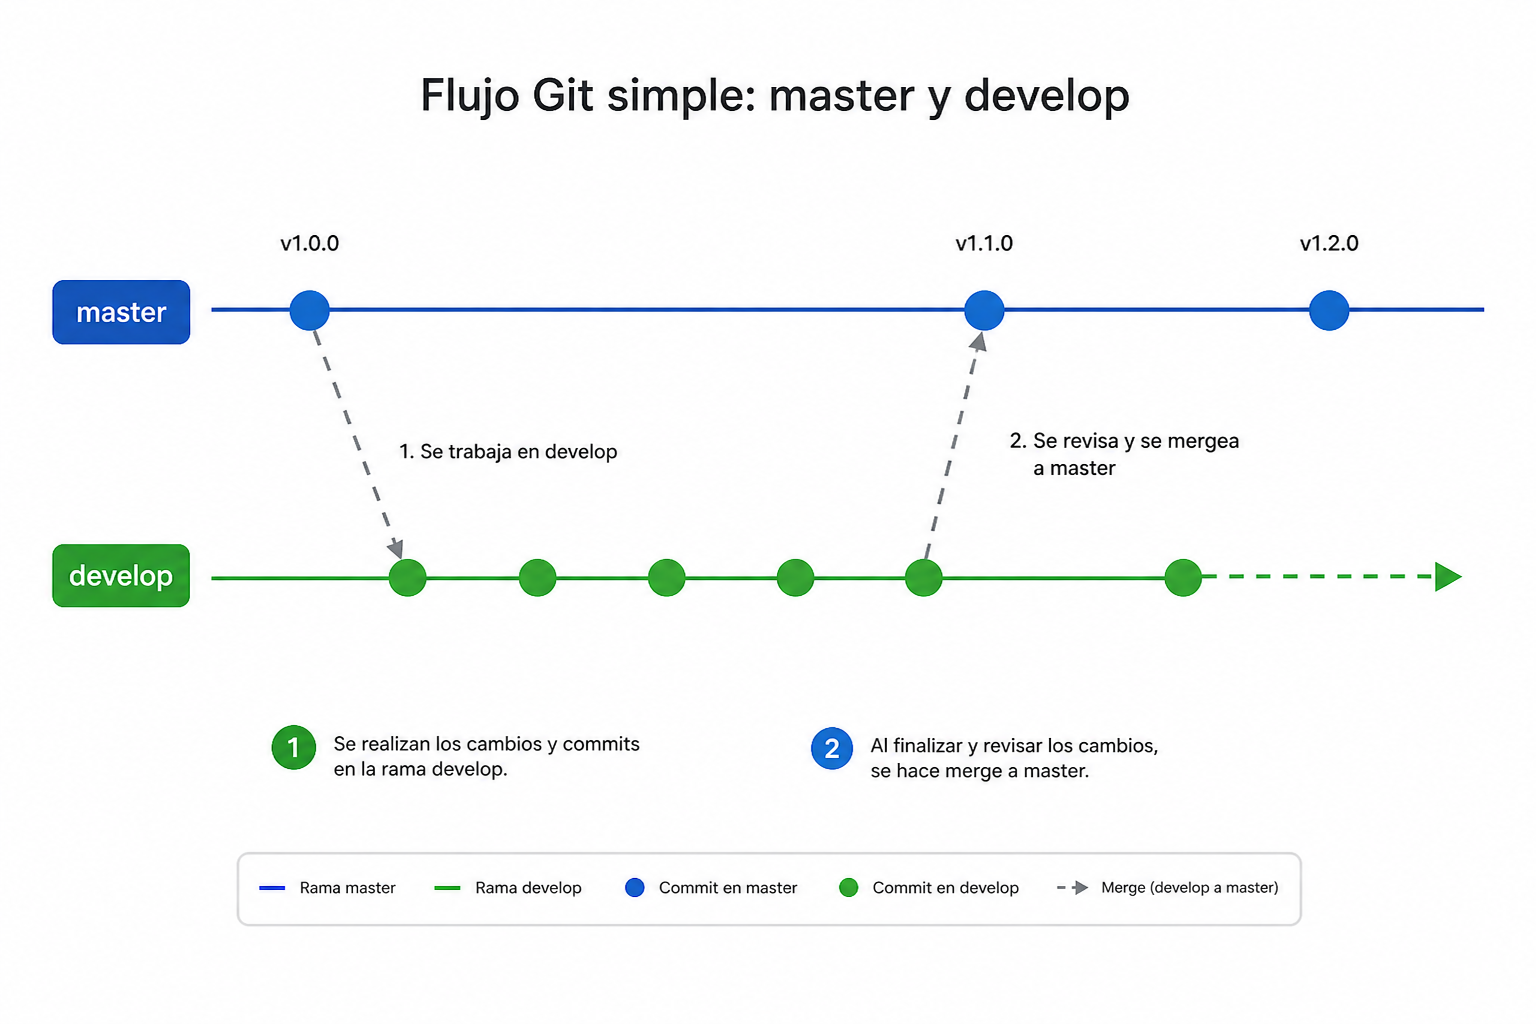
\includegraphics[width=0.95\textwidth]{figures/figura_4_1_workflow.png}
    \caption{Modelo de ramificación utilizado en GlucoMate: rama \texttt{develop} para
             integración continua y \texttt{master} para versiones estables.}
    \label{fig:git-workflow}
\end{figure}

% ──────────────────────────────────────────────────────────────
\section{Conventional Commits}
\label{sec:conventional-commits}

Para garantizar que el historial de \textit{commits} sea legible, semántico y
automáticamente procesable, todos los mensajes de confirmación de cambios siguen la
especificación \textbf{Conventional Commits} \cite{conventionalcommits}, una convención
ampliamente adoptada en la industria del software.

\subsection{Estructura del mensaje}

Cada mensaje de \textit{commit} responde a la siguiente estructura:

\begin{verbatim}
<tipo>(<ámbito>): <descripción breve>

[cuerpo opcional]

[notas de pie opcionales]
\end{verbatim}

\noindent Donde \texttt{<tipo>} es uno de los valores definidos por la especificación:

\begin{table}[H]
\centering
\caption{Tipos de \textit{commit} utilizados en GlucoMate según la especificación
         Conventional Commits.}
\label{tab:commit-types}
\begin{tabular}{|l|p{9.5cm}|}
\hline
\textbf{Tipo} & \textbf{Significado} \\
\hline
\texttt{feat}     & Añade una nueva funcionalidad al sistema. \\
\texttt{fix}      & Corrige un error o comportamiento incorrecto. \\
\texttt{refactor} & Reestructura código sin cambiar su comportamiento externo. \\
\texttt{docs}     & Cambios exclusivamente en la documentación. \\
\texttt{style}    & Ajustes de formato, sangría o estilo sin impacto funcional. \\
\texttt{chore}    & Tareas de mantenimiento: actualización de dependencias, configuración. \\
\texttt{test}     & Adición o modificación de pruebas. \\
\texttt{perf}     & Mejora del rendimiento de algún componente. \\
\hline
\end{tabular}
\end{table}

\subsection{Ejemplos representativos del proyecto}

A continuación se recogen mensajes de \textit{commit} reales del historial de GlucoMate
que ilustran la aplicación de esta convención:

\begin{verbatim}
fix(ui): corregir posición inicial del trazado en la gráfica.
feat(ui): implementar e integrar el modal de registro de insulina.
feat(api): añadir endpoints para gestionar eventos de insulina.
chore: actualizar dependencias en package.json.
feat(ui): añadir assets para los botones de acción.
Merge pull request #2 from manortgar/develop
chore: actualizar .gitignore
fix(ui): ajustar dimensiones de pantalla al área segura de Android.
Merge pull request #1 from manortgar/develop
feat(ui): implementa vista de Mi Perfil de usuario y nueva ruta.
chore(brand): cambiar nombre de la aplicación e icono.
feat(api): añadir nuevos endpoints para la gestión de Mi Perfil.
\end{verbatim}

\subsection{Beneficios obtenidos}

La adopción de esta convención ha aportado tres beneficios concretos al proyecto:

\begin{enumerate}
    \item \textbf{Legibilidad del historial.} Cualquier persona que consulte el
          repositorio puede entender qué cambió, en qué capa del sistema y con qué
          intención, sin necesidad de leer el \textit{diff} completo.

    \item \textbf{Generación automática de \textit{changelogs}.} Herramientas como
          \texttt{standard-version} o \texttt{release-please} pueden generar un
          registro de cambios estructurado a partir de los mensajes de \textit{commit},
          lo que facilitará las versiones futuras de la aplicación.

    \item \textbf{Disciplina de desarrollo.} La obligación de clasificar cada
          \textit{commit} fuerza al desarrollador a realizar cambios atómicos y con
          una responsabilidad clara, evitando los \textit{commits} de tipo
          ``arreglos varios'' que dificultan la revisión y la depuración.
\end{enumerate}

% ──────────────────────────────────────────────────────────────
\section{Buenas prácticas aplicadas}
\label{sec:buenas-practicas}

Más allá del control de versiones, el desarrollo de GlucoMate ha incorporado un conjunto
de buenas prácticas de ingeniería de software que se describen a continuación.

\subsection{Separación de responsabilidades: arquitectura cliente-servidor}
\label{subsec:separacion-responsabilidades}

El sistema está dividido en dos capas claramente diferenciadas —\textbf{frontend} y
\textbf{backend}— que se comunican exclusivamente a través de una API REST documentada.
Esta separación garantiza que:

\begin{itemize}
    \item La lógica de negocio (cálculo de IOB, integración con Groq y
          \texttt{llama-3.3-70b-versatile}, gestión de transacciones en base de datos)
          reside en el servidor, donde puede ser
          mantenida y actualizada sin redistribuir la aplicación móvil.
    \item El cliente móvil se limita a presentar datos y gestionar la interacción con el
          usuario, sin acoplar lógica de dominio en los componentes de interfaz.
    \item Ambas capas pueden evolucionar de forma independiente: un futuro cliente web
          o iOS podría consumir la misma API sin modificar el backend.
\end{itemize}

\subsection{Modularidad y cohesión}
\label{subsec:modularidad}

El frontend está organizado en componentes React Native con responsabilidades únicas y
bien definidas:

\begin{itemize}
    \item \textbf{\texttt{NFCScanner.js}}: pantalla principal. Gestiona el estado global
          de la aplicación (lectura NFC, historial, eventos activos) y orquesta el
          renderizado de la gráfica y los módulos de acción.
    \item \textbf{\texttt{ChatModal.js}}: interfaz de conversación con el agente de IA.
          Completamente autocontenido, recibe \texttt{backendUrl} como argumento y gestiona
          su propio estado de mensajes y carga.
    \item \textbf{\texttt{InsulinModal.js}, \texttt{FoodModal.js},
          \texttt{ExerciseModal.js}}: modales de registro de eventos clínicos. Cada uno
          encapsula su formulario, validación y llamada al \textit{endpoint} correspondiente.
    \item \textbf{\texttt{ProfileScreen.js}}: pantalla de perfil. Independiente del flujo
          principal, gestiona la carga y persistencia del perfil de tratamiento.
\end{itemize}

En el backend, la separación entre \texttt{server.js} (lógica de rutas y controladores)
y \texttt{db.js} (gestión del \textit{pool} de conexiones a PostgreSQL) sigue el principio
de responsabilidad única (SRP) y facilita la sustitución del motor de base de datos sin
tocar la lógica de negocio.

\subsection{Gestión de errores y resiliencia}
\label{subsec:gestion-errores}

El backend implementa un mecanismo de \textbf{reintento con espera exponencial} para las
llamadas a la API de Groq, dado que este servicio puede responder con errores 503
(\textit{Service Unavailable}) o 429 (\textit{Too Many Requests}) bajo carga. El
algoritmo realiza hasta tres intentos con una pausa de cinco segundos entre ellos antes
de propagar el error al cliente:

\begin{lstlisting}[language=JavaScript, caption={Mecanismo de reintento con espera exponencial
para las llamadas a la API de Groq}, label={cod:error-ia}, captionpos=b]
let retries = 3;
while (retries > 0 && !success) {
    try {
        response = await ai.models.generateContent({ ... });
        success = true;
    } catch (err) {
        if ((err.status === 503 || err.status === 429) && retries > 1) {
            retries--;
            await new Promise(resolve => setTimeout(resolve, 5000));
        } else {
            throw err;
        }
    }
}
\end{lstlisting}

Adicionalmente, todas las rutas del backend están envueltas en bloques \texttt{try/catch}
que devuelven respuestas HTTP con códigos de estado apropiados (400, 500) y mensajes
descriptivos, evitando que un error interno exponga información sensible del sistema.

Las operaciones que implican múltiples escrituras en la base de datos —como el registro
de una comida con bolo de insulina asociado— se ejecutan dentro de
\textbf{transacciones ACID} con \texttt{BEGIN}/\texttt{COMMIT}/\texttt{ROLLBACK},
garantizando la consistencia de los datos ante fallos parciales.

\subsection{Variables de entorno y seguridad de credenciales}
\label{subsec:env-vars}

Las credenciales sensibles del sistema (clave de API de Groq, contraseña de PostgreSQL,
host y puerto de la base de datos) se gestionan mediante \textbf{variables de entorno}
cargadas con la librería \texttt{dotenv}. El fichero \texttt{.env} está incluido en
\texttt{.gitignore} para garantizar que nunca se publique en el repositorio:

\begin{verbatim}
# .env (nunca versionado)
GROQ_API_KEY=gsk_...
DB_USER=postgres
DB_PASSWORD=...
DB_NAME=glucose_db
DB_HOST=localhost
DB_PORT=5432
\end{verbatim}

Esta práctica es especialmente crítica en proyectos que integran APIs de terceros con
facturación por uso, donde una clave comprometida podría derivar en costes económicos
significativos.

\subsection{Arquitectura de la API REST}
\label{subsec:api-rest}

Los \textit{endpoints} del backend siguen las convenciones REST estándar: sustantivos
en plural para los recursos, verbos HTTP semánticos (\texttt{GET} para consulta,
\texttt{POST} para creación, \texttt{PUT} para actualización completa) y códigos de
estado HTTP coherentes con el resultado de cada operación (201 para creación exitosa,
400 para validación fallida, 500 para error interno). Esta consistencia facilita el
consumo de la API desde el cliente y, en el futuro, desde cualquier otra aplicación.

% ──────────────────────────────────────────────────────────────
\section{Gestión de dependencias con npm y build con EAS}
\label{sec:herramientas}

La selección de tecnologías ha respondido a tres criterios: adecuación técnica al
problema, madurez del ecosistema y productividad en un contexto de desarrollo individual.

\subsection{React Native con Expo}
\label{subsec:herramienta-rn}

\textbf{React Native} \cite{facebook2015reactnative} es un \textit{framework} de código
abierto desarrollado por Meta que permite construir aplicaciones móviles nativas para
Android e iOS utilizando JavaScript y el paradigma de componentes de React. A diferencia
de las soluciones de \textit{webview} (como Ionic o Cordova), React Native compila los
componentes a elementos de interfaz nativos de cada plataforma, lo que proporciona
rendimiento y aspecto visual indistinguibles de una aplicación nativa.

La elección de React Native sobre alternativas como Flutter o el desarrollo nativo en
Kotlin/Java se justifica por:

\begin{itemize}
    \item La disponibilidad de \texttt{react-native-nfc-manager}, una librería madura
          que abstrae el acceso a la pila NFC del sistema operativo Android y soporta el
          protocolo ISO 15693 (NfcV) necesario para comunicarse con el sensor Freestyle
          Libre.
    \item El ecosistema JavaScript compartido con el backend (Node.js), que reduce la
          carga cognitiva de cambiar de lenguaje entre capas.
    \item La reutilización de librerías de visualización como D3.js, cuyo ecosistema es
          incomparablemente más rico en JavaScript que en Dart o Kotlin.
\end{itemize}

\textbf{Expo} \cite{expo2020} es una plataforma construida sobre React Native que
simplifica la configuración del entorno de desarrollo, la gestión de permisos del sistema
operativo (NFC, cámara, etc.) y el proceso de compilación. En GlucoMate se utiliza con
la configuración \texttt{expo-dev-client}, que permite generar una aplicación de
desarrollo personalizada con acceso completo a las APIs nativas, superando las
limitaciones de la versión estándar de Expo Go para funcionalidades como NFC.

\subsection{Build de producción con EAS Build}
\label{subsec:herramienta-eas}

\textbf{EAS Build} (Expo Application Services Build) \cite{eas2021} es el servicio de
compilación en la nube de Expo. Permite generar el APK o AAB de producción de la
aplicación Android sin necesidad de tener instalado Android Studio ni el SDK de Android
en la máquina local. La configuración del proyecto en \texttt{eas.json} define los
perfiles de compilación (\textit{development}, \textit{preview}, \textit{production})
con sus respectivas opciones de firma y distribución.

La justificación de EAS Build frente a la compilación local es doble: elimina la
complejidad de mantener una cadena de compilación nativa en el entorno de desarrollo y
garantiza reproducibilidad en entornos limpios y controlados.

\subsection{Gestión de dependencias con npm}
\label{subsec:herramienta-npm}

\textbf{npm} (\textit{Node Package Manager}) \cite{npm2010} es el gestor de paquetes
estándar del ecosistema JavaScript, utilizado tanto en el frontend como en el backend. El
fichero \texttt{package-lock.json} garantiza que las instalaciones sean reproducibles,
fijando las versiones exactas de todas las dependencias transitivas. Entre las bibliotecas
más relevantes del frontend se encuentran \texttt{react-native-nfc-manager} para el acceso
al hardware NFC, \texttt{d3-shape} y \texttt{d3-scale} para la representación de curvas y
escalas temporales, \texttt{react-native-svg} para el renderizado gráfico y
\texttt{@react-navigation/bottom-tabs} para la navegación principal de la aplicación.

En el backend, las dependencias clave incluyen \texttt{express} como marco HTTP,
\texttt{pg} para la conexión con PostgreSQL, el SDK de Groq para el acceso al modelo
\texttt{llama-3.3-70b-versatile}, además de utilidades como \texttt{dotenv} para la carga
de configuración y \texttt{cors} para habilitar la comunicación segura con el cliente móvil.

\subsection{Backend: Node.js con Express}
\label{subsec:herramienta-node}

\textbf{Node.js} \cite{nodejs2009} es un entorno de ejecución JavaScript asíncrono
basado en el motor V8 de Google Chrome, diseñado para construir aplicaciones de red
escalables. Su modelo de E/S no bloqueante mediante \textit{event loop} lo hace
especialmente adecuado para APIs REST que realizan operaciones de I/O intensivas
(consultas a base de datos, llamadas a APIs externas), que es exactamente el perfil
de carga de GlucoMate.

\textbf{Express} \cite{express2010} es el \textit{framework} HTTP minimalista más
utilizado en el ecosistema Node.js. Proporciona un sistema de enrutamiento, \textit{middleware}
y gestión de peticiones/respuestas HTTP con una superficie de API reducida, lo que facilita
la comprensión y el mantenimiento del código del servidor.

\subsection{Base de datos: PostgreSQL}
\label{subsec:herramienta-postgres}

\textbf{PostgreSQL} \cite{postgres1996} es el sistema de gestión de bases de datos
relacionales de código abierto más avanzado disponible. Su elección sobre alternativas
como SQLite o MySQL se justifica por:

\begin{itemize}
    \item \textbf{Soporte completo de ACID.} Las transacciones del backend que registran
          simultáneamente una comida y un bolo de insulina requieren garantías de
          atomicidad que SQLite no ofrece de forma robusta en escenarios concurrentes.
    \item \textbf{Tipos de datos ricos.} PostgreSQL soporta \texttt{TIMESTAMP WITH TIME
          ZONE}, \texttt{NUMERIC} y \texttt{INTERVAL} de forma nativa, lo que simplifica
          las consultas de ventana temporal (por ejemplo, ``lecturas de las últimas 12 horas'').
    \item \textbf{UPSERT nativo.} La instrucción \texttt{INSERT ... ON CONFLICT DO UPDATE}
          permite gestionar el perfil de usuario como una fila única que se crea o
          actualiza atómicamente, sin necesidad de lógica adicional en el servidor.
    \item \textbf{Escalabilidad futura.} Aunque en la versión actual el backend opera en
          red local, PostgreSQL está preparado para ser desplegado en entornos de
          producción en la nube (AWS RDS, Supabase) sin cambios en el esquema ni en el
          código de acceso a datos.
\end{itemize}

\subsection{Visualización: D3.js sobre SVG nativo}
\label{subsec:herramienta-d3}

\textbf{D3.js} (\textit{Data-Driven Documents}) \cite{bostock2011d3} es la librería de
visualización de datos más utilizada en el ecosistema JavaScript. En GlucoMate se emplean
específicamente los módulos \texttt{d3-scale} y \texttt{d3-shape}, que proporcionan:

\begin{itemize}
    \item \texttt{scaleTime()}: transforma marcas de tiempo Unix en coordenadas
          de píxel en el eje X, gestionando correctamente los cambios de horario y
          la aritmética de fechas.
    \item \texttt{scaleLinear()}: mapea los valores de glucosa (rango 50–300+ mg/dL)
          al eje Y del área de dibujo.
    \item \texttt{line().curve(curveMonotoneX)}: genera la ruta SVG de la curva
          interpolada con suavizado monotónico, que preserva la forma real de los datos
          sin introducir oscilaciones artificiales entre puntos.
\end{itemize}

La elección de D3.js sobre librerías de gráficas de alto nivel para React Native
(Victory Native, React Native Chart Kit) se justifica por el nivel de control que
requiere la gráfica de GlucoMate: la superposición de múltiples capas de información
(curva de glucosa, ventanas de insulina activa con línea de pico, ventanas de ejercicio
con zona de peligro postejercicio, marcadores de comidas) es una visualización altamente
personalizada que las librerías de gráficas estándar no permiten implementar sin
comprometer su API interna.

\subsection{Inteligencia Artificial: \texttt{llama-3.3-70b-versatile} en Groq}
\label{subsec:herramienta-llama-groq}

El agente de inteligencia artificial de GlucoMate está construido sobre
\textbf{\texttt{llama-3.3-70b-versatile}} \cite{groq2026llama}, un modelo de lenguaje
grande (LLM) servido a través de la API de Groq. La elección de esta combinación frente
a alternativas como GPT-4o (OpenAI) o Claude (Anthropic) se fundamenta en:

\begin{itemize}
    \item \textbf{Latencia.} Groq está orientado a inferencia de baja latencia,
          lo que es esencial en una aplicación móvil donde el usuario espera una
          respuesta en tiempo real.
    \item \textbf{Coste.} El acceso gratuito mediante una API key de Groq es suficiente para el
          volumen de consultas de un usuario individual, lo que hace viable el proyecto
          sin coste operativo.
    \item \textbf{Temperatura baja.} El modelo se configura con \texttt{temperature: 0.2},
          lo que reduce la variabilidad de las respuestas y favorece el razonamiento
          clínico estructurado frente a respuestas creativas.
\end{itemize}

La integración se realiza en el backend (no en el cliente móvil), lo que garantiza que
la clave de API nunca se expone en el código de la aplicación distribuida.

\subsection{Prototipado: mockups digitales}
\label{subsec:herramienta-prototipado}

El diseño de la interfaz de usuario se abordó mediante \textbf{mockups digitales de
alta fidelidad} antes de cerrar la implementación visual definitiva. Este enfoque
permitió validar con antelación la jerarquía visual, el reparto del espacio y la
consistencia cromática de la aplicación, además de comunicar con claridad la propuesta
de interfaz sin necesidad de desarrollar todavía todos los flujos funcionales.

Los mockups definieron las decisiones de diseño más importantes de la interfaz: la
disposición del valor de glucosa como elemento dominante en la parte superior de la
pantalla, la ubicación del botón NFC en la esquina superior izquierda para acceso rápido,
la fila de botones de acción rápida (comida, insulina, deporte) como acceso directo a
los modales de registro, la pantalla de perfil terapéutico para la configuración del
tratamiento y el acceso al chat de IA en posición secundaria pero visible.

Las Figuras~\ref{fig:mockups-ui-principales} y~\ref{fig:mockups-ui-secundarias}
recogen los mockups principales elaborados para el proyecto: la pantalla principal con
la curva glucémica, la vista de perfil terapéutico, los formularios de registro de
eventos y la interfaz conversacional del asistente.

\newcommand{\mockupcard}[2]{%
    \begin{tikzpicture}
        \node[inner sep=0pt, outer sep=0pt] (img) at (0,0)
            {\includegraphics[width=#1,height=0.36\textheight,keepaspectratio]{#2}};
        \begin{scope}
            \clip[rounded corners=7pt] (img.south west) rectangle (img.north east);
            \node[inner sep=0pt, outer sep=0pt, anchor=south west] at (img.south west)
                {\includegraphics[width=#1,height=0.36\textheight,keepaspectratio]{#2}};
        \end{scope}
        \draw[rounded corners=7pt, line width=0.45pt, draw=black!25]
            (img.south west) rectangle (img.north east);
    \end{tikzpicture}%
}

\begin{figure}[p]
    \centering
    \subfigure[Pantalla principal con lectura actual de glucosa, accesos rápidos y gráfica histórica.]{%
        \mockupcard{0.78\textwidth}{uploads/grafica4-3.png}}

    \vspace{1em}

    \subfigure[Pantalla de perfil terapéutico para la configuración de insulinas e ICR.]{%
        \mockupcard{0.78\textwidth}{uploads/perfil4-3.png}}
    \caption{Mockups principales de la interfaz de GlucoMate.}
    \label{fig:mockups-ui-principales}
\end{figure}

\begin{figure}[p]
    \centering
    \subfigure[Formularios de registro de comida, insulina y deporte mediante modales específicos.]{%
        \mockupcard{0.78\textwidth}{uploads/Copilot_20260510_131939.png}}

    \vspace{1em}

    \subfigure[Interfaz conversacional del asistente GlucoMate AI para apoyo y orientación contextual.]{%
        \mockupcard{0.78\textwidth}{uploads/chat4-3.png}}
    \caption{Mockups complementarios de interacción y asistencia inteligente.}
    \label{fig:mockups-ui-secundarias}
\end{figure}

% ──────────────────────────────────────────────────────────────
\section{Resumen}
\label{sec:metodologia-resumen}

La tabla~\ref{tab:resumen-metodologia} sintetiza las decisiones metodológicas y
tecnológicas más relevantes del proyecto.

\begin{table}[H]
\centering
\caption{Resumen de la metodología y tecnologías principales de GlucoMate.}
\label{tab:resumen-metodologia}
\begin{tabular}{|l|l|}
\hline
\textbf{Dimensión} & \textbf{Decisión adoptada} \\
\hline
Metodología       & Desarrollo ágil iterativo (iteraciones semanales) \\
Control versiones & Git + GitHub (\texttt{develop} / \texttt{master}) \\
Estilo de commits & Conventional Commits \\
Frontend          & React Native 0.81 + Expo 54 \\
Build nativo      & EAS Build (Expo Application Services) \\
Gestor paquetes   & npm + \texttt{package-lock.json} \\
Visualización     & D3.js (\texttt{d3-scale}, \texttt{d3-shape}) + react-native-svg \\
Backend           & Node.js + Express 5 \\
Base de datos     & PostgreSQL (pool de conexiones con \texttt{pg}) \\
IA generativa     & \texttt{llama-3.3-70b-versatile} (Groq, \texttt{temperature: 0.2}) \\
Seguridad         & Variables de entorno con \texttt{dotenv} \\
Prototipado UI    & Mockups digitales de alta fidelidad \\
Plataforma target & Android (API 24+) \\
\hline
\end{tabular}
\end{table}

    % ============================================================
%  CAPÍTULO 5 — DISEÑO DE LA SOLUCIÓN
%  TFG: GlucoMate — Aplicación de Monitorización Continua de Glucosa
%  Ingeniería de Software
% ============================================================

\chapter{Diseño de la Solución}
\label{cap:diseno}

Este capítulo describe las decisiones de diseño que dan forma al sistema GlucoMate:
la arquitectura general, la descomposición en módulos, el esquema de base de datos,
el diseño de la API REST, la visualización de datos y el diseño del agente de
inteligencia artificial.

% ──────────────────────────────────────────────────────────────
\section{Arquitectura general del sistema}
\label{sec:arquitectura-general}

GlucoMate sigue una \textbf{arquitectura cliente-servidor en tres capas} que separa
de forma limpia la presentación, la lógica de negocio y el almacenamiento de datos.
La figura~\ref{fig:arquitectura-general} muestra el diagrama completo del sistema
con todos sus componentes y los canales de comunicación entre ellos.

\begin{figure}[H]
\centering
\resizebox{0.88\textwidth}{!}{%
\begin{tikzpicture}[
    box/.style={draw, rounded corners, align=center, minimum width=2.9cm, minimum height=0.9cm, font=\small},
    ext/.style={box, fill=orange!12, draw=orange!70!black},
    app/.style={box, fill=blue!10, draw=blue!60!black},
    srv/.style={box, fill=green!10, draw=green!50!black},
    db/.style={box, fill=gray!15, draw=black!60},
    label/.style={font=\scriptsize, fill=white, inner sep=1pt}
]
    \node[ext] (sensor) at (0,0) {Sensor\\Freestyle Libre 2 Plus};
    \node[ext] (juggluco) at (0,-1.8) {Juggluco\\puente local};
    \node[app] (frontend) at (0,-3.6) {Frontend móvil\\React Native + Expo};
    \node[srv] (backend) at (-3.6,-5.6) {Backend REST\\Node.js + Express};
    \node[db] (postgres) at (3.6,-5.6) {PostgreSQL\\persistencia};
    \node[ext] (llama) at (0,-7.3) {\texttt{llama-3.3-70b-versatile}\\Groq API};
    \draw[-{Latex[length=2.6mm]}, thick] (sensor) -- node[label, right] {BLE / NFC} (juggluco);
    \draw[-{Latex[length=2.6mm]}, thick] (juggluco) -- node[label, right] {HTTP local} (frontend);
    \draw[-{Latex[length=2.6mm]}, thick] (frontend) -- node[label, below left] {API REST} (backend);
    \draw[-{Latex[length=2.6mm]}, thick] (frontend) -- node[label, below right] {histórico} (postgres);
    \draw[-{Latex[length=2.6mm]}, thick] (backend) -- node[label, below] {SQL} (postgres);
    \draw[-{Latex[length=2.6mm]}, thick] (backend) -- node[label, left] {prompt} (llama);
\end{tikzpicture}%
}

\caption{Arquitectura general del sistema GlucoMate. El sensor se comunica con
         Juggluco por BLE; el frontend obtiene los datos vía HTTP local y los
         persiste a través de la API REST; el backend accede a PostgreSQL y a
         la API de Groq para consumir el modelo \texttt{llama-3.3-70b-versatile}.}
\label{fig:arquitectura-general}
\end{figure}

\noindent La arquitectura presenta las siguientes características destacables:

\begin{itemize}
    \item \textbf{Desacoplamiento completo entre capas.} El frontend no accede
          directamente a la base de datos; toda la lógica de datos pasa por la
          API REST del backend. Esto permite actualizar el esquema de base de
          datos sin modificar el cliente.

    \item \textbf{Juggluco como puente de seguridad.} El sensor Freestyle Libre 2
          Plus utiliza un enlace BLE cifrado con claves derivadas del número de
          serie del sensor. Juggluco gestiona ese descifrado y expone los datos
          ya procesados en mg/dL a través de un servidor HTTP en \texttt{localhost},
          eliminando la necesidad de reimplementar la criptografía propietaria de
          Abbott en GlucoMate.

    \item \textbf{IA en el backend.} La integración con Groq y el modelo
          \texttt{llama-3.3-70b-versatile} se realiza
          exclusivamente en el servidor, garantizando que la clave de API nunca
          se distribuye con el APK de la aplicación.

    \item \textbf{Operación en red local.} En la versión actual, el frontend y el
          backend operan en la misma red Wi-Fi local, con la IP del servidor
          configurada estáticamente. Esto es suficiente para la validación del
          prototipo y establece las bases para una futura migración a infraestructura
          en la nube.
\end{itemize}

% ──────────────────────────────────────────────────────────────
\section{Diseño de la aplicación móvil (React Native + Expo)}
\label{sec:arquitectura-frontend}

El frontend de GlucoMate está estructurado como una \textbf{Single Screen Application
con navegación por pestañas}, implementada con \texttt{@react-navigation/bottom-tabs}.
La figura~\ref{fig:arquitectura-frontend} muestra la jerarquía de componentes.

\begin{figure}[H]
\centering
\resizebox{0.92\textwidth}{!}{%
\begin{tikzpicture}[
    comp/.style={draw, rounded corners, align=center, minimum width=2.6cm, minimum height=0.8cm, font=\small},
    root/.style={comp, fill=blue!10, draw=blue!60!black},
    screen/.style={comp, fill=green!10, draw=green!50!black},
    child/.style={comp, fill=gray!10, draw=black!55, minimum width=2.4cm, minimum height=0.62cm, font=\scriptsize}
]
    \node[root] (app) at (0,0) {App.js\\NavigationContainer};
    \node[screen] (glucose) at (-4.0,-1.9) {Pestaña Glucosa\\\texttt{NFCScanner.js}};
    \node[screen] (profile) at (4.0,-1.9) {Pestaña Mi Perfil\\\texttt{ProfileScreen.js}};
    \node[child] (graph) at (-8.4,-3.7) {renderGraph + D3};
    \node[child] (food) at (-4.0,-3.7) {FoodModal};
    \node[child] (exercise) at (-0.6,-3.7) {ExerciseModal};
    \node[child] (chat) at (-6.4,-5.5) {ChatModal};
    \node[child] (insulin) at (-2.0,-5.5) {InsulinModal};
    \node[child] (picker) at (2.0,-4.7) {Selector de insulinas};
    \node[child] (icr) at (4.0,-3.7) {Ratios ICR};
    \node[child] (fsi) at (6.0,-4.7) {Factor FSI};
    \draw[-{Latex[length=2.4mm]}, thick] (app.south west) -- (glucose.north);
    \draw[-{Latex[length=2.4mm]}, thick] (app.south east) -- (profile.north);
    \draw[-{Latex[length=2.2mm]}, thick] (glucose.south west) -- (graph.north);
    \draw[-{Latex[length=2.2mm]}, thick] (glucose.south) -- (food.north);
    \draw[-{Latex[length=2.2mm]}, thick] (glucose.south east) -- (exercise.north);
    \draw[-{Latex[length=2.2mm]}, thick] (glucose.south east) -- (insulin.north);
    \draw[-{Latex[length=2.2mm]}, thick] (glucose.south west) -- (chat.north);
    \draw[-{Latex[length=2.2mm]}, thick] (profile.south west) -- (picker.north);
    \draw[-{Latex[length=2.2mm]}, thick] (profile.south) -- (icr.north);
    \draw[-{Latex[length=2.2mm]}, thick] (profile.south east) -- (fsi.north);
\end{tikzpicture}%
}
\caption{Jerarquía de componentes del frontend de GlucoMate.}
\label{fig:arquitectura-frontend}
\end{figure}

\texttt{NFCScanner.js} actúa como el \textbf{componente raíz de la pestaña principal}
y concentra la mayor parte del estado de la aplicación mediante los hooks de React
\texttt{useState} y \texttt{useEffect}. Es el responsable de:

\begin{itemize}
    \item Inicializar el gestor NFC al montar el componente y cancelar la solicitud
          de tecnología al desmontar, evitando fugas de recursos.
    \item Cargar el historial de glucosa, el perfil de usuario y los eventos clínicos
          de las últimas 12 horas en paralelo.
    \item Orquestar el flujo de escaneo NFC → llamada a Juggluco → persistencia en
          backend → recarga de historial.
    \item Gestionar la visibilidad de los cuatro modales (insulina, comida, ejercicio,
          chat IA) mediante flags.
\end{itemize}

% ──────────────────────────────────────────────────────────────
\section{Diseño de la base de datos}
\label{sec:diseno-bd}

El esquema de la base de datos PostgreSQL está diseñado para modelar los conceptos
clínicos relevantes en el autocontrol de la diabetes tipo 1: lecturas de glucosa,
perfil de tratamiento individual, eventos de insulina, comidas y ejercicio.

\subsection{Diagrama Entidad-Relación}
\label{subsec:er-diagram}

\begin{figure}[H]
\centering
\resizebox{0.92\textwidth}{!}{%
\begin{tikzpicture}[
    entity/.style={draw, rounded corners, align=left, minimum width=2.7cm, text width=2.5cm, font=\scriptsize, inner sep=4pt},
    rel/.style={-{Latex[length=2.2mm]}, thick}
]
    \node[entity, fill=blue!8] (glucose) at (-4.2,0) {\textbf{glucose\_readings}\\id (PK)\\user\_id\\glucose\_value\\trend\\reading\_time\\created\_at};
    \node[entity, fill=green!8] (profile) at (0,0) {\textbf{user\_profile}\\id (PK)\\fast\_insulin\_id\\slow\_insulin\_id\\ICR + FSI\\updated\_at};
    \node[entity, fill=yellow!10] (insulins) at (4.2,0) {\textbf{insulins}\\id (PK)\\name\\type\\duration\_hours\\peak\_hours};
    \node[entity, fill=orange!10] (food) at (-4.2,-3.1) {\textbf{food\_events}\\id (PK)\\user\_id\\carbs\_g\\event\_time\\created\_at};
    \node[entity, fill=orange!10] (insEvents) at (0,-3.1) {\textbf{insulin\_events}\\id (PK)\\user\_id\\insulin\_id\\units\\event\_time\\created\_at};
    \node[entity, fill=orange!10] (exercise) at (4.2,-3.1) {\textbf{exercise\_events}\\id (PK)\\user\_id\\sport\_id\\start\_time\\duration\_minutes\\created\_at};
    \node[entity, fill=purple!10] (sports) at (4.2,-6.0) {\textbf{sports}\\id (PK)\\name\\intensity\_type\\danger\_window};
    \draw[rel] (profile) -- node[above, font=\scriptsize] {configura} (insulins);
    \draw[rel] (insEvents) -- node[right, font=\scriptsize] {usa} (insulins);
    \draw[rel] (exercise) -- node[right, font=\scriptsize] {usa} (sports);
    \draw[rel] (glucose) -- node[above, font=\scriptsize] {contexto} (profile);
    \draw[rel] (food) -- node[above, font=\scriptsize] {registro} (insEvents);
\end{tikzpicture}%
}
\caption{Diagrama entidad-relación simplificado del esquema de base de datos de
         GlucoMate.}
\label{fig:er-diagram}
\end{figure}

\subsection{Descripción de las tablas}
\label{subsec:tablas}

\begin{description}
    \item[\texttt{glucose\_readings}] Almacena cada lectura de glucosa recibida del
    sensor. El campo \texttt{trend} recoge la dirección de la tendencia tal como la
    reporta Juggluco (\texttt{Flat}, \texttt{SingleUp}, \texttt{FortyFiveDown}, etc.),
    y \texttt{reading\_time} es un \texttt{TIMESTAMP} que permite las consultas de
    ventana temporal (\texttt{NOW() - INTERVAL '12 HOURS'}) usadas por la gráfica.

    \item[\texttt{insulins}] Catálogo de insulinas conocidas, con su tipo
    (\texttt{fast}/\texttt{slow}), duración total en horas (\texttt{duration\_hours}) y
    hora de pico de acción (\texttt{peak\_hours}). Esta tabla es referenciada por
    \texttt{user\_profile} y por \texttt{insulin\_events}, y sus valores se utilizan
    en la gráfica para calcular las ventanas de insulina activa.

    \item[\texttt{user\_profile}] Contiene exactamente una fila (con \texttt{id = 1})
    que representa el perfil de tratamiento del usuario. Los campos \texttt{icr\_*}
    son los ratios insulina-carbohidrato para cada franja horaria del día
    (desayuno, media mañana, almuerzo, merienda y cena), y \texttt{fsi} es el
    Factor de Sensibilidad a la Insulina (mg/dL por unidad). La tabla se gestiona
    mediante un \texttt{UPSERT} (\texttt{INSERT ... ON CONFLICT DO UPDATE}) que
    garantiza que siempre existe una única fila, independientemente del número de
    veces que se guarde el perfil.

    \item[\texttt{insulin\_events}] Registra cada inyección de insulina realizada por
    el usuario. La clave foránea \texttt{insulin\_id} permite conocer la duración y el
    pico de cada dosis, datos necesarios para calcular la insulina activa (IOB) y para
    renderizar las ventanas rosas en la gráfica.

    \item[\texttt{food\_events}] Registra cada comida con sus gramos de carbohidratos
    y la hora de ingesta. Esta información aparece en la gráfica como marcadores
    verdes con la cantidad de hidratos, y es el dato de entrada principal para el
    cálculo de dosis del agente de IA.

    \item[\texttt{sports}] Catálogo de actividades deportivas con su tipo de
    intensidad (\texttt{Aeróbico}, \texttt{Mixto}, \texttt{Baja intensidad},
    \texttt{Anaeróbico}) y su ventana de peligro en horas
    (\texttt{danger\_window\_hours}), que determina cuánto tiempo después del
    ejercicio puede seguir afectando a la glucosa.

    \item[\texttt{exercise\_events}] Registra cada sesión de ejercicio con su
    deporte, hora de inicio y duración en minutos. Esta información se usa tanto
    para la representación gráfica (ventana naranja con línea de peligro
    postejercicio punteada) como para el contexto del agente de IA, que aplica
    reducciones de bolo en función del tipo de intensidad del deporte.
\end{description}

\subsection{Decisiones de diseño relevantes de la BD}
\label{subsec:decisiones-bd}

\begin{itemize}
    \item \textbf{Perfil de usuario como fila única.} El diseño de \texttt{user\_profile}
          con \texttt{id = 1} fijo es una simplificación deliberada para un sistema
          monousuario. El mecanismo \texttt{UPSERT} garantiza que la pantalla de perfil
          siempre opera correctamente, tanto en la primera configuración como en
          actualizaciones posteriores.

    \item \textbf{Catálogos de insulinas y deportes.} Separar las propiedades
          farmacológicas de las insulinas (duración, pico) y las características de los
          deportes (intensidad, ventana de peligro) en tablas de catálogo independientes
          permite que el sistema sea extensible: añadir una nueva insulina o un nuevo
          deporte no requiere cambios en la lógica de la aplicación.

    \item \textbf{Transacción atómica en registro de comida.} Cuando el usuario
          registra una comida e indica también un bolo de insulina, el backend ejecuta
          ambas inserciones (\texttt{food\_events} e \texttt{insulin\_events}) dentro
          de una misma transacción. Si cualquiera de las dos falla, se hace
          \texttt{ROLLBACK} completo, garantizando que nunca quede una comida registrada
          sin su insulina asociada ni viceversa.
\end{itemize}

% ──────────────────────────────────────────────────────────────
\section{Diseño de la API REST}
\label{sec:diseno-api}

El backend expone una API REST que constituye el único canal de comunicación entre
el frontend y los datos. La tabla~\ref{tab:api-endpoints} recoge todos los
\textit{endpoints} implementados.

\begin{table}[H]
\centering
\caption{Endpoints de la API REST de GlucoMate.}
\label{tab:api-endpoints}
\begin{tabular}{|l|l|p{7cm}|}
\hline
\textbf{Método} & \textbf{Ruta} & \textbf{Descripción} \\
\hline
\texttt{POST} & \texttt{/api/glucose}            & Persiste una nueva lectura de glucosa (valor, tendencia, timestamp). \\
\texttt{GET}  & \texttt{/api/glucose/history}    & Devuelve las lecturas de las últimas 12 horas ordenadas por tiempo, para la gráfica D3. \\
\hline
\texttt{GET}  & \texttt{/api/insulins}           & Devuelve el catálogo completo de insulinas (rápidas y lentas). \\
\texttt{GET}  & \texttt{/api/profile}            & Devuelve el perfil de tratamiento del usuario (JOIN con insulinas). \\
\texttt{PUT}  & \texttt{/api/profile}            & Crea o actualiza el perfil de tratamiento (UPSERT). \\
\hline
\texttt{GET}  & \texttt{/api/insulin-events}     & Devuelve inyecciones de insulina recientes (parámetro \texttt{hours}, por defecto 24). \\
\texttt{POST} & \texttt{/api/insulin-events}     & Registra una nueva inyección de insulina. \\
\hline
\texttt{GET}  & \texttt{/api/food-events}        & Devuelve comidas registradas recientes (parámetro \texttt{hours}). \\
\texttt{POST} & \texttt{/api/food-events}        & Registra una comida y, opcionalmente, el bolo de insulina asociado (transacción). \\
\hline
\texttt{GET}  & \texttt{/api/sports}             & Devuelve el catálogo de deportes disponibles. \\
\texttt{GET}  & \texttt{/api/exercise-events}    & Devuelve sesiones de ejercicio recientes. \\
\texttt{POST} & \texttt{/api/exercise-events}    & Registra una nueva sesión de ejercicio. \\
\hline
\texttt{POST} & \texttt{/api/chat}               & Envía un mensaje al agente de IA. Recopila contexto en tiempo real, construye el \textit{system prompt} y llama a Groq para inferir con \texttt{llama-3.3-70b-versatile}. \\
\hline
\end{tabular}
\end{table}

Todos los \textit{endpoints} de escritura aceptan y devuelven JSON con cabecera
\texttt{Content-Type: application/json}. Las respuestas de error incluyen siempre un
campo \texttt{error} con un mensaje descriptivo y un código HTTP apropiado (400 para
errores de validación, 500 para errores internos del servidor).

% ──────────────────────────────────────────────────────────────
\section{Decisiones de diseño}
\label{sec:diseno-grafica}

La gráfica de glucosa es el elemento central de la interfaz de GlucoMate y el que
mayor complejidad de diseño presenta. Se han tomado las siguientes decisiones de diseño:

\subsection{Ventana temporal y escalas}
\label{subsec:ventana-temporal}

La gráfica muestra siempre una ventana de \textbf{12 horas}: 11 horas hacia el pasado
desde el momento actual y 1 hora hacia el futuro. Esta decisión reproduce la convención
clínica establecida por las principales aplicaciones de MCG (Dexcom CLARITY, LibreLinkUp)
y permite al usuario ver la tendencia reciente con suficiente contexto histórico.

Las escalas se calculan dinámicamente en cada renderizado:

\begin{itemize}
    \item \textbf{Eje X (temporal):} \texttt{d3Scale.scaleTime()} mapea el rango de
          timestamps [\texttt{ahora - 11h}, \texttt{ahora + 1h}] al ancho de pantalla
          en píxeles, con un margen lateral de 20px en cada extremo.

    \item \textbf{Eje Y (glucosa):} \texttt{d3Scale.scaleLinear()} mapea el rango
          [50, \texttt{max\_12h + 50}] a la altura del SVG, con el valor mínimo fijo
          en 50 mg/dL y el máximo calculado dinámicamente como el pico del historial
          más un margen de 50 mg/dL para evitar que la curva toque el borde superior.
\end{itemize}

\subsection{Curva de glucosa}
\label{subsec:curva}

La curva principal se genera con \texttt{d3Shape.line().curve(d3Shape.curveMonotoneX)},
que produce una interpolación cúbica monotónica. Esta elección sobre otras curvas de D3
(cardinal, catmull-rom, natural) se justifica porque \texttt{curveMonotoneX} garantiza
que la curva no oscila artificialmente entre puntos: si los datos van hacia arriba, la
curva va hacia arriba, lo que es crítico en un contexto clínico donde una oscilación
falsa podría malinterpretarse como un evento real de hipoglucemia o hiperglucemia.

\subsection{Líneas de referencia clínicas}
\label{subsec:lineas-referencia}

La gráfica incluye dos líneas horizontales de referencia punteadas en los valores
\textbf{70 mg/dL} (umbral de hipoglucemia) y \textbf{180 mg/dL} (umbral de
hiperglucemia), con la zona entre ellas coloreada en verde translúcido
(\texttt{rgba(200, 230, 201, 0.4)}) como indicador visual del rango objetivo.
Estos valores son los estándares clínicos reconocidos por la American Diabetes
Association (ADA).

\subsection{Capas de eventos superpuestas}
\label{subsec:capas-eventos}

Una de las características más innovadoras de la gráfica de GlucoMate es la
superposición de múltiples capas de información clínica sobre la curva de glucosa.
El diseño contempla tres capas independientes, cada una activable/desactivable
mediante los \textit{chips} de filtro:

\begin{description}
    \item[\textbf{Capa de insulina rápida (rosa).}] Para cada inyección de insulina
    rápida activa, se dibuja un rectángulo translúcido (\texttt{rgba(255, 105, 180, 0.3)})
    que abarca desde el momento de la inyección hasta el fin de su duración. Una línea
    vertical punteada de color rosa intenso (\texttt{\#e91e63}) marca el momento de
    pico de acción de la insulina, el instante en que su efecto hipoglucemiante es
    máximo.

    \item[\textbf{Capa de ejercicio (naranja).}] Para cada sesión de ejercicio, se
    dibuja un rectángulo translúcido (\texttt{rgba(255, 152, 0, 0.3)}) durante la
    duración de la actividad. Una línea punteada naranja horizontal indica la
    extensión de la ventana de peligro postejercicio (\texttt{danger\_window\_hours}),
    el periodo durante el cual el ejercicio sigue afectando a la sensibilidad a la
    insulina.

    \item[\textbf{Capa de comidas (verde).}] Cada comida se representa con un
    marcador circular verde en la parte inferior de la gráfica, mostrando los gramos
    de carbohidratos registrados, y una línea vertical punteada que sube hasta la
    parte superior del área de dibujo.


\end{description}

Una capa superpuesta sobre la gráfica pero siempre visible y no desactivable es las\textbf{etiquetas de eje X.} Los ticks del eje temporal se muestran cada
    dos horas en horas pares (00:00, 02:00, 04:00...), calculadas de forma dinámica
    para que siempre sean horas redondas independientemente del momento del día.

\subsection{Indicador de glucosa actual}
\label{subsec:indicador-glucosa}

El valor actual de glucosa se muestra con una tipografía de \textbf{110 puntos} en la
parte superior de la pantalla, coloreado dinámicamente según el rango:

\begin{itemize}
    \item \textcolor{blue}{\textbf{Azul}} (\texttt{\#2196F3}): glucosa en rango normal (70--180 mg/dL).
    \item \textcolor{red}{\textbf{Rojo}} (\texttt{\#f44336}): hipoglucemia (menor a 70 mg/dL).
    \item \textcolor{orange}{\textbf{Naranja}} (\texttt{\#ff9800}): hiperglucemia (mayor a 180 mg/dL).
    \item \textbf{Gris} (\texttt{\#9e9e9e}): dato antiguo o sin lectura reciente.
\end{itemize}

La flecha de tendencia (\texttt{up / up-right / right / down-right / down}) se renderiza con una fuente
personalizada (\texttt{ArrowFont}) cargada mediante \texttt{expo-font}, ya que los
caracteres de flecha estándar de Unicode no tienen representación tipográfica uniforme
en todos los dispositivos Android.

% ──────────────────────────────────────────────────────────────
\section{Diseño de la capa de presentación (UI/UX)}
\label{sec:diseno-modales}

Los tres modales de registro de eventos clínicos (insulina, comida y ejercicio) siguen
un patrón de diseño uniforme:

\begin{enumerate}
    \item \textbf{Modal superpuesto con overlay semitransparente.} Cada modal se
          presenta como un \texttt{Modal} de React Native con \texttt{transparent=true}
          y un overlay \texttt{rgba(0,0,0,0.5)} que oscurece el contenido subyacente,
          manteniendo el contexto visual de la pantalla principal.

    \item \textbf{Selector de hora manual.} Los tres modales incluyen un selector
          de hora compuesto por dos campos \texttt{TextInput} (horas y minutos),
          inicializados con la hora actual del dispositivo. Si la hora introducida
          es posterior a la hora actual del sistema, el modal la interpreta
          automáticamente como perteneciente al día anterior, resolviendo el caso
          de uso habitual de registrar una inyección nocturna antes de medianoche.

    \item \textbf{Feedback visual de estado.} El botón de guardar muestra un
          \texttt{ActivityIndicator} durante el guardado y queda deshabilitado
          hasta que los campos obligatorios son válidos, previniendo envíos duplicados.
\end{enumerate}

Las particularidades de cada modal son:

\begin{description}
    \item[\texttt{InsulinModal.js}] Permite seleccionar entre insulina rápida e
    insulina lenta mediante un selector de dos botones cuyo estado activo muestra
    los colores específicos de cada tipo (rosa para rápida, morado para lenta),
    tomando los nombres de insulina configurados en el perfil del usuario.

    \item[\texttt{FoodModal.js}] Incluye dos campos numéricos: gramos de
    carbohidratos y unidades de bolo de insulina rápida. El campo de bolo queda
    deshabilitado si el usuario no tiene insulina rápida configurada en su perfil,
    mostrando un mensaje de error orientativo.

    \item[\texttt{ExerciseModal.js}] Carga dinámicamente el catálogo de deportes
    desde el \textit{endpoint} \texttt{/api/sports} al abrirse, mostrando cada
    deporte junto con su ventana de peligro en horas. El formulario incluye también
    la duración de la sesión en minutos.
\end{description}

% ──────────────────────────────────────────────────────────────
\section{Diseño del perfil de usuario y parametrización clínica}
\label{sec:diseno-perfil}

La pantalla \texttt{ProfileScreen.js} permite al usuario configurar los parámetros
individuales de su tratamiento, que el agente de IA utilizará como contexto para
personalizar sus recomendaciones.

Los parámetros configurables son:

\begin{itemize}
    \item \textbf{Insulina rápida y lenta:} seleccionadas mediante \texttt{Picker}
          desplegable del catálogo de insulinas, mostrando nombre y duración (7 insulinas rápidas y 6 lentas, guardadas en base de datos. Las más comunes).
    \item \textbf{Ratios ICR por franja horaria:} un campo numérico por cada una de
          las cinco franjas del día (desayuno, media mañana, almuerzo, merienda y cena),
          expresado en gramos de carbohidratos por unidad de insulina (g/U).
    \item \textbf{Factor de Sensibilidad a la Insulina (FSI):} cuántos mg/dL reduce
          la glucosa una unidad de insulina rápida, utilizado para calcular el bolo
          de corrección cuando la glucosa está por encima del rango.
\end{itemize}

El guardado se realiza mediante una petición \texttt{PUT} a \texttt{/api/profile},
que ejecuta un \texttt{UPSERT} en la base de datos. El botón de guardar cambia
visualmente a verde con el texto ``Guardado correctamente'' durante 3 segundos tras una
operación exitosa, o a rojo con ``Error al guardar'' si la petición falla, antes
de volver a su estado neutro.

% ──────────────────────────────────────────────────────────────
\section{Diseño del agente de IA (lógica de recomendación según perfil)}
\label{sec:diseno-ia}

El agente de IA de GlucoMate es el componente más innovador del sistema. Su diseño
se basa en el paradigma de \textbf{\textit{context-aware prompting}}: en lugar de
enviar al modelo únicamente el mensaje del usuario, el backend construye en tiempo
real un \textit{system prompt} rico en datos clínicos del usuario antes de cada
llamada a la API.

\subsection{Recolección de contexto en tiempo real}
\label{subsec:contexto-ia}

Al recibir una petición \texttt{POST /api/chat}, el backend ejecuta cuatro consultas
SQL en paralelo mediante \texttt{Promise.all}:

\begin{enumerate}
    \item \textbf{Perfil de tratamiento:} ratios ICR por franja horaria y FSI.
    \item \textbf{Insulina activa (IOB):} suma de unidades de insulina rápida
          inyectadas en las últimas 4 horas.
    \item \textbf{Ejercicio en ventana de peligro:} deportes practicados cuya
          ventana de peligro aún no ha expirado, con su tipo de intensidad.
    \item \textbf{Glucosa actual:} último valor registrado y su tendencia.
\end{enumerate}

La ejecución en paralelo minimiza la latencia total de recopilación de contexto,
que de otro modo se acumularía de forma secuencial.

\subsection{Lógica de reducción por tipo de deporte}
\label{subsec:reduccion-deporte}

El sistema implementa una tabla de reducción de bolo en función del tipo de
intensidad del ejercicio practicado:

\begin{table}[H]
\centering
\caption{Porcentajes de reducción del bolo de insulina por tipo de intensidad
         deportiva, implementados en la constante \texttt{SPORT\_REDUCTION} del backend.}
\label{tab:sport-reduction}
\begin{tabular}{|l|c|p{6cm}|}
\hline
\textbf{Tipo de intensidad} & \textbf{Reducción} & \textbf{Comportamiento del agente} \\
\hline
Aeróbico        & 20\%  & Reduce el bolo calculado y lo explica. \\
Mixto           & 12,5\% & Reduce el bolo calculado y lo explica. \\
Baja intensidad & 5\%   & Reduce el bolo calculado y lo explica. \\
Anaeróbico      & 0\%   & No reduce el bolo, pero advierte del riesgo de hipoglucemia postejercicio. \\
\hline
\end{tabular}
\end{table}

Si el usuario ha practicado múltiples deportes en sus respectivas ventanas de peligro,
el sistema aplica la reducción máxima de entre todos ellos. Si alguno es anaeróbico,
se emite la advertencia correspondiente adicionalmente.

\subsection{Construcción del \textit{system prompt}}
\label{subsec:system-prompt}

El \textit{system prompt} que recibe \texttt{llama-3.3-70b-versatile} en cada llamada es un documento de texto
estructurado en secciones que incluye:

\begin{itemize}
    \item \textbf{Identidad y restricciones:} el agente se identifica como
          ``GlucoMate AI'', responde siempre en español y de forma concisa.
    \item \textbf{Datos en tiempo real:} glucosa actual, tendencia, ICR por franja
          horaria, FSI, y alerta de IOB activo si supera 1 UI.
    \item \textbf{Instrucciones de cálculo de bolo:} algoritmo paso a paso con
          fórmula explícita (\texttt{unidades = (g HC ÷ 10) × ICR}), con instrucción
          de solicitar la franja horaria si no está clara.
    \item \textbf{Reglas de glucosa actual:} si la glucosa es menor de 70, no
          recomendar insulina; si es mayor de 180, añadir bolo de corrección
          (\texttt{(glucosa - 100) ÷ FSI}); si está en rango, sin corrección.
    \item \textbf{Contexto de deporte:} la reducción de bolo calculada o la
          advertencia de deporte anaeróbico.
    \item \textbf{Aviso obligatorio:} el agente debe incluir al inicio de cada
          respuesta el texto ``Aviso: soy una IA de apoyo, no un médico. Esta sugerencia
          no reemplaza el criterio clínico.'', garantizando que el usuario siempre
          conoce las limitaciones del sistema.
\end{itemize}

El modelo se llama con \texttt{temperature: 0.2} para maximizar la consistencia
y el rigor del razonamiento clínico, minimizando la variabilidad creativa que
sería inapropiada en un contexto médico.

\subsection{Mecanismo de reintento}
\label{subsec:reintento-ia}

La llamada a la API de Groq está protegida por un mecanismo de reintento que
realiza hasta 3 intentos con una pausa de 5 segundos entre ellos ante errores 503
(\textit{Service Unavailable}) o 429 (\textit{Too Many Requests}). Cualquier otro
tipo de error se propaga inmediatamente al cliente.

% ──────────────────────────────────────────────────────────────
\section{Diseño de la interfaz de usuario}
\label{sec:diseno-ui}

El diseño visual de GlucoMate parte de los mockups digitales elaborados durante la
fase de prototipado y sigue los principios del \textit{Material Design} de Google,
que es la referencia de diseño nativa de Android.

Las decisiones de diseño más relevantes son:

\begin{itemize}
    \item \textbf{Jerarquía visual clara.} El valor de glucosa (110pt) domina
          visualmente la pantalla, ya que es la información más crítica para el
          usuario diabético. Los demás elementos (gráfica, botones de acción) se
          subordinan a él en tamaño e importancia visual.

    \item \textbf{Codificación de color semántica y consistente.} El sistema usa
          el mismo código de color en toda la interfaz: verde para comidas, rosa/rojo
          para insulina rápida, morado para insulina lenta, naranja para ejercicio.
          Esta consistencia permite al usuario interpretar la gráfica de forma
          intuitiva sin necesidad de leer etiquetas.

    \item \textbf{Botón NFC en posición de pulgar.} El botón de escaneo se sitúa
          en la esquina superior izquierda de la pantalla, zona de máxima
          accesibilidad con el pulgar derecho en dispositivos de pantalla grande.
          Cambia de color a naranja mientras espera el escaneo, proporcionando
          feedback visual inmediato del estado del sistema.

    \item \textbf{Navegación por pestañas inferior.} La barra de navegación
          inferior con dos pestañas (Glucosa y Mi Perfil) sigue el patrón de
          navegación estándar de Android y respeta el área segura del sistema
          mediante \texttt{useSafeAreaInsets}, evitando solapamientos con la
          barra de navegación del sistema.

    \item \textbf{Botón flotante de IA (FAB).} El acceso al chat de inteligencia
          artificial se implementa como un botón flotante de acción (FAB) de color
          azul marino (\texttt{\#1a237e}) con un icono de chispa (\texttt{sparkles}),
          que evoca la naturaleza inteligente de la funcionalidad sin ocupar espacio
          permanente en la interfaz principal.
\end{itemize}

% ──────────────────────────────────────────────────────────────
\section{Flujo global de interacción}
\label{sec:flujo-principal}

El flujo de uso más frecuente de GlucoMate —escanear el sensor y consultar al
agente de IA— sigue la siguiente secuencia:

\begin{figure}[H]
\centering
\resizebox{0.92\textwidth}{!}{%
\begin{tikzpicture}[
    lifeline/.style={font=\small, align=center},
    msg/.style={-{Latex[length=2.2mm]}, thick},
    reply/.style={msg, dashed},
    every node/.style={font=\scriptsize}
]
    \node[lifeline] (u) at (0,0) {Usuario};
    \node[lifeline] (f) at (3.4,0) {Frontend};
    \node[lifeline] (b) at (6.8,0) {Backend};
    \node[lifeline] (g) at (10.2,0) {Groq / BD};
    \foreach \x in {u,f,b,g} \draw[densely dashed] (\x.south) -- ++(0,-10.4);
    \draw[msg] (0,-0.8) -- node[above] {Pulsa NFC} (3.4,-0.8);
    \draw[msg] (3.4,-1.5) -- node[above] {NfcV} (6.8,-1.5);
    \draw[reply] (6.8,-2.2) -- node[above] {activo} (3.4,-2.2);
    \draw[msg] (3.4,-2.9) -- node[above] {GET Juggluco} (6.8,-2.9);
    \draw[reply] (6.8,-3.6) -- node[above] {lectura} (3.4,-3.6);
    \draw[msg] (3.4,-4.3) -- node[above] {POST /glucose} (6.8,-4.3);
    \draw[msg] (6.8,-5.0) -- node[above] {persistencia} (10.2,-5.0);
    \draw[reply] (10.2,-5.7) -- node[above] {ok + histórico} (6.8,-5.7);
    \draw[reply] (6.8,-6.4) -- node[above] {gráfica} (3.4,-6.4);
    \draw[msg] (0,-7.1) -- node[above] {consulta IA} (3.4,-7.1);
    \draw[msg] (3.4,-7.8) -- node[above] {POST /chat} (6.8,-7.8);
    \draw[msg] (6.8,-8.5) -- node[above] {prompt + contexto} (10.2,-8.5);
    \draw[reply] (10.2,-9.2) -- node[above] {respuesta} (6.8,-9.2);
    \draw[reply] (6.8,-9.9) -- node[above] {reply} (3.4,-9.9);
\end{tikzpicture}%
}
\caption{Diagrama de secuencia del flujo principal de GlucoMate: escaneo NFC y
         consulta al agente de IA.}
\label{fig:flujo-principal}
\end{figure}

    \chapter{Pruebas}\label{cap:pruebas}

\section{Estrategia de pruebas}

La validación de este sistema debía combinar pruebas funcionales manuales, verificación del
flujo de datos entre frontend y backend y comprobaciones de usabilidad sobre la interfaz.
Dado que el proyecto depende de hardware real, la estrategia de pruebas debe contemplar
tanto escenarios controlados de laboratorio como pruebas de uso cotidiano.

En un sistema como GlucoMate no bastaba con verificar funciones aisladas. Es necesario
comprobar una cadena completa que incluye hardware, conectividad local, backend, base de
datos y renderizado en interfaz. Por ello, la estrategia más realista para este TFG es la
de prueba funcional de integración, complementada con comprobaciones manuales sobre cada
módulo: lectura de glucosa, registro de eventos, persistencia y asistencia por IA.

\section{Pruebas funcionales con sensor real Freestyle Libre}

Las pruebas funcionales más relevantes son las realizadas con un sensor real y un teléfono
Android con soporte NFC. La secuencia de validación adecuada para este proyecto puede
resumirse en los siguientes pasos:

\begin{enumerate}
    \item Abrir la aplicación móvil y verificar la carga del histórico, el perfil y los
          eventos clínicos recientes. \textbf{EXITOSA}
    \item Activar el flujo de escaneo NFC, aproximar el teléfono al sensor y que se detecte comprobando así el uso del chip NFC. \textbf{EXITOSA}
    \item Confirmar que el frontend obtiene una lectura válida desde el puente Juggluco. \textbf{EXITOSA}
    \item Verificar que la lectura se almacena correctamente en el backend y aparece en el
          histórico de 12 horas. \textbf{EXITOSA}
    \item Registrar una comida, una dosis de insulina y una actividad deportiva, y
          comprobar su reflejo inmediato en la interfaz. \textbf{EXITOSA}
    \item Enviar una consulta al agente de IA y validar que la respuesta utiliza el
          contexto clínico reciente. \textbf{EXITOSA}
\end{enumerate}

Este enfoque permitió comprobar no solo la funcionalidad de cada módulo, sino también la
coherencia temporal entre ellos, que es un aspecto esencial del sistema.

\section{Resultados y evidencias}

Los resultados obtenidos durante las pruebas confirman que el flujo principal de
GlucoMate se ejecuta correctamente de extremo a extremo. La aplicación es capaz de recibir
las lecturas procedentes del sensor, mostrarlas en la interfaz y mantenerlas sincronizadas
con el resto de módulos del sistema. En las comprobaciones realizadas, los valores de
glucosa recibidos por la aplicación coinciden con los valores que se pueden visualizar en
la aplicación oficial Abbott FreeStyle LibreLink, lo que permite validar que la lectura
integrada en GlucoMate conserva la información original del sensor sin alterar su valor
clínico ni su marca temporal.

Esta verificación se ha realizado comparando manualmente la lectura mostrada en GlucoMate
con la lectura visible en LibreLink para el mismo instante de medición. La coincidencia
entre ambas aplicaciones demuestra que el sistema interpreta correctamente los datos
recibidos y que el frontend representa de forma fiel la información capturada. Además, la
gráfica histórica y la lectura actual mantienen una evolución coherente, sin saltos
temporales injustificados ni discrepancias entre el dato puntual mostrado al usuario y el
histórico almacenado.

La persistencia en base de datos también se comporta de forma correcta. Cada lectura,
evento de comida, dosis de insulina, actividad física o registro clínico se almacena con
una marca temporal asociada, permitiendo reconstruir la secuencia de acontecimientos de
manera ordenada. Las pruebas realizadas evidencian que los datos guardados conservan
coherencia temporal entre sí y que, tras cerrar y volver a abrir la aplicación, la
información continúa disponible y se muestra de forma consistente en el frontend. Por
tanto, no se trata únicamente de una visualización temporal en la interfaz, sino de una
persistencia efectiva en el backend.

Las evidencias principales de este apartado se apoyan en tres elementos: capturas de la
pantalla principal con la lectura actual y la gráfica histórica, comprobaciones de la base
de datos con los registros persistidos y comparación directa con la aplicación oficial
Abbott FreeStyle LibreLink. En conjunto, estas evidencias permiten afirmar que el sistema
funciona de forma estable, que los datos se guardan correctamente y que existe coherencia
entre el sensor, la base de datos y la información presentada al usuario en la aplicación.



    \chapter{Conclusiones y trabajo futuro}\label{cap:conclusiones}

\section{Conclusiones}

GlucoMate demuestra que es posible construir, en el contexto de un Trabajo de Fin de
Grado, un prototipo funcional capaz de integrar captura de glucosa, registro clínico,
persistencia estructurada y asistencia contextual en una única aplicación móvil. La
aportación principal del proyecto no reside únicamente en haber desarrollado una interfaz
atractiva, sino en haber conectado varias capas tecnológicas heterogéneas en un flujo
coherente: sensor, aplicación puente, frontend móvil, backend, base de datos y agente de
IA.

Desde el punto de vista de la ingeniería del software, el proyecto ha permitido abordar
problemas reales de arquitectura, modularidad, comunicación cliente-servidor y gestión de
estado en un dominio especialmente exigente por su sensibilidad clínica. Además, la
decisión de separar claramente frontend y backend ha resultado adecuada para proteger
credenciales, estructurar la lógica de negocio y mantener una base razonable para futuras
evoluciones.

También es relevante el valor práctico del sistema desarrollado. Frente a soluciones que
se limitan a mostrar lecturas de glucosa aisladas, GlucoMate propone una visión más rica
del problema: relaciona glucosa, insulina, alimentación y actividad deportiva, y utiliza
ese contexto para ofrecer apoyo interpretativo al usuario. Aunque la aplicación no pretende
sustituir el criterio médico ni alcanzar el nivel de un producto sanitario certificado, sí
evidencia el potencial de las herramientas software personalizadas en la gestión cotidiana
de la diabetes tipo 1.

\section{Objetivos alcanzados}


Se cumplieron todos los objetivos planteados al inicio del proyecto. Se integró correctamente la lectura de datos del sensor mediante NFC, utilizando \textit{Juggluco} como puente para el descifrado de la señal BLE. Además, se desarrolló un backend REST con Node.js, Express y PostgreSQL para la gestión y almacenamiento de lecturas glucémicas y eventos clínicos.

Asimismo, se implementó una interfaz gráfica capaz de representar de forma clara la evolución histórica de la glucosa junto con los eventos clínicos asociados. También se desarrolló un agente de inteligencia artificial basado en \textit{llama-3.3-70b-versatile}, capaz de ofrecer recomendaciones personalizadas y cálculos orientativos de dosis de insulina en función del contexto clínico del usuario.

Por otro lado, se diseñó una pantalla de perfil que permitió configurar los parámetros individuales de tratamiento, haciendo posible una mayor personalización del sistema.

Finalmente, la validación con un sensor real en un dispositivo Android físico confirmó el correcto funcionamiento de la solución desarrollada.

En conclusión, este trabajo demostró la viabilidad de combinar tecnologías móviles, sistemas backend e inteligencia artificial para crear herramientas de apoyo al control glucémico, sentando una base sólida para futuras mejoras y ampliaciones del sistema.
\section{Líneas de trabajo futuro}

Las principales líneas de evolución previstas para GlucoMate incluyen la ampliación a
iOS, la mejora de los algoritmos de recomendación mediante modelos de IA más avanzados y
la migración desde una arquitectura local a un backend desplegado en la nube.

Además de estas líneas generales, existen varias mejoras concretas especialmente
interesantes para una continuación del proyecto:

\begin{itemize}
    \item \textbf{Despliegue en la nube:} sustituir la IP fija en red local por una
          infraestructura estable, segura y accesible desde distintos entornos.
    \item \textbf{Ampliación de métricas:} incorporar indicadores como Tiempo en Rango,
          glucosa media estimada o métricas agregadas por franjas temporales.
    \item \textbf{Mejora del agente de IA:} enriquecer el contexto, refinar los prompts y
          estudiar mecanismos de validación o trazabilidad de recomendaciones. Correr un modelo propio entrenado con datos específicos de diabetes en una máquina o servidor privado.
    \item \textbf{Mayor automatización de pruebas:} añadir pruebas de backend, validaciones
          de API y mecanismos de verificación más sistemáticos.
    \item \textbf{Integración multiplataforma:} explorar las limitaciones reales de iOS y
          estudiar alternativas técnicas compatibles con el ecosistema Apple.
     \item \textbf{Rentabilización mediante patrocinios:} estudiar un modelo de
          sostenibilidad económica basado en acuerdos con fabricantes de sensores
          compatibles, actualmente Abbott, y con compañías farmacéuticas relacionadas con
          la producción de insulinas, como Novo Nordisk, Eli Lilly o Sanofi. Este enfoque
          permitiría financiar la evolución técnica, el mantenimiento de la infraestructura
          y posibles procesos de validación, manteniendo como principio fundamental que el
          usuario final no tuviera que asumir ningún coste por utilizar la aplicación.
\end{itemize}

En conjunto, estas líneas muestran que el trabajo realizado no cierra el proyecto, pero sí
establece una base sólida y realista sobre la que seguir construyendo una herramienta cada
vez más útil, robusta y cercana a un entorno de uso real y lo más importante, ayudando cada día mas a los millones de diabeticos que necesitan una ayuda en su tratamiento diario.


    % Bibliografía
    \bibliographystyle{unsrtnat}
    \bibliography{bibliografia.bib}
        

% Fin del documento
\end{document}
